\chapter{Partielle differensialligninger}
\label{sect:PDE}

Partielle differensialligninger (PDE) oppstår ofte i formuleringen av naturens grunnleggende lover og i den matematiske analysen av et bredt spekter av problemer innen anvendt matematikk, matematisk fysikk og ingeniørvitenskap. Dette spiller en sentral rolle i moderne matematiske vitenskaper, spesielt innen fysikk. Mange problemer av fysisk interesse beskrives ved hjelp av PDE med passende initial- og/eller randbetingelser. Disse problemene formuleres vanligvis som initialverdiproblemer, randverdiproblemer eller initial-randverdiproblemer. Generelle kilder for materialet som fremstilles i kapittelet er \cite{Deb12,LaT03}.

\textbf{Jeg har hørt at PDE er super vanskelig!} Det stemmer hvis man leter etter en generell metode for å finne eksakte løsninger for dem. Vi skal gjøre noe som er mye enklere: Beskrive hvordan PDE oppstår i anvendelser, se på noen typer og lære oss hvordan vi kan finne gode tilnærminger til løsninger ved hjelp av datamaskiner. 

\section{Introduksjon til PDE}\label{sect:introPDE}

En partiell differensialligning (PDE) for en funksjon \( u(x, y, \ldots) \) er et forhold mellom \( u \) og dens partielle deriverte \( u_x, u_y, u_{xx}, u_{xy}, u_{yy}, \ldots \), og kan skrives som
\begin{align}\label{eq:PDE1}
F(x, y, u, u_x, u_y, u_{xx}, u_{xy}, u_{yy}, \ldots) = 0, 
\end{align}
der \( F \) er en funksjon og \( x, y, \ldots \) er uavhengige variable. Videre kalles \( u(x, y, \ldots) \) avhengig variabel. En funksjon $u$ kalles en løsning til \eqref{eq:PDE1} dersom den er tilstrekkelig deriverbar og oppfyller \eqref{eq:PDE1}.

Ordenen til en partiell differensialligning defineres, i likhet med ordinære differensialligninger, som den høyeste ordenen av deriverte som opptrer i likningen. Den mest generelle førsteordens partielle differensialligning kan skrives som
\begin{align}\label{eq:fo_PDE}
F(x, y, u, u_x, u_y) = 0. 
\end{align}
Som eksempel er følgende likninger alle 1.ordens PDEer.
\begin{equation}\label{eq:ex_fo_PDEs} \begin{aligned}
x u_x + y u_y = 0.\\
x u_x + y u_y = x^2 + y^2, \\
u u_x + u_t = u, \\
u_x^2 + u_y^2 = 1 \end{aligned}
\end{equation}
Tilsvarende har den mest generelle andreordens partielle differensialligningen i to uavhengige variable \( x, y \) formen
\begin{align}\label{eq:so_PDE}
F(x, y, u, u_x, u_y, u_{xx}, u_{xy}, u_{yy}) = 0,
\end{align}
Tilsvarende relasjoner kan selvsagt skrives ned for ligninger av høyere orden. Eksempler på 2.ordens ligninger er
\begin{equation}\label{eq:ex_so_PDEs}
\begin{aligned}u_{xx} + 2u_{xy} + u_{yy} = 0,\\
u_{xx} + u_{yy} = 0, \\
u_{tt} - c^2 u_{xx} + \sin(u)= f(x, t).\end{aligned}
\end{equation}


\begin{defn}{}
En PDE \eqref{eq:PDE1} kalles 
\begin{itemize}
\item \emph{lineær} dersom den er lineær i den ukjente funksjonen og alle dens deriverte, med koeffisienter som kun avhenger av de uavhengige variablene.
\item \emph{kvasi-lineær} dersom den er lineær i den høyeste ordenen til den ukjente funksjonens deriverte.
\end{itemize}
Som i teorien for ordinære differensiallikninger (ODE) kan man alltid skrive \eqref{eq:PDE1} om slik at høyresiden kun inneholder uavhengige variable, $f(x,y,\ldots)$, mens venstresiden avhenger av $u$ i tillegg. Derson $f(x,y,\ldots)=0$ kaller vi likningen \emph{homogen}, ellers er den inhomogen.
\end{defn}

Noen eksempler:
\begin{table}[ht]
\centering
\begin{tabular}{|c|c|c|c|}
\hline
       & lineær  & kvasi-lineær & ikke-lineær \\
\hline
homogen  &  1 i \eqref{eq:ex_fo_PDEs}, 1 og 2 i \eqref{eq:ex_so_PDEs} & $u_{xx}+uu_t =0$ & $u_{xx}^2-u_{yy}^2=0$\\
\hline
inhomogen  & 2 i \eqref{eq:ex_fo_PDEs} & 3 i \eqref{eq:ex_so_PDEs}  & 4 i \eqref{eq:ex_fo_PDEs}\\
\hline
\end{tabular}
\caption{Klassifisering av PDE}
\label{tab:example}
\end{table}

La oss præve å løse en enkel ligning for \( u = u(x, y) \):
\begin{align}\label{eq:ex_PDE2}
u_{xy} = 0. 
\end{align}
Ved å integrere denne ligningen med hensyn på \( x \), får vi $u_y = h(y)$, hvor \( h(y) \) er en vilkårlig funksjon av \( y \). Vi integrerer deretter med hensyn på \( y \) for å finne
$u(x, y) = \int h(y)\,dy + f(x)$ 
hvor \( f(x) \) er en vilkårlig funksjon. Eller ekvivalent,
\begin{align}\label{eq:sol1}
u(x, y) = f(x) + g(y),
\end{align}
hvor \( f(x) \) og \( g(y) \) er vilkårlige funksjoner.

\begin{defn}{}
Løsningen \eqref{eq:sol1} kalles den \emph{generelle løsningen} av den andreordens ligningen \eqref{eq:ex_PDE2}.
\end{defn}
Vanligvis er den generelle løsningen av en partiell differensialligning et uttrykk som inneholder vilkårlige funksjoner i sterk kontrast til den generelle løsningen av en ODE, som typisk inneholdt vilkårlige \textit{konstanter.}

Videre har \eqref{eq:ex_PDE2} uendelig mange løsninger. Dette kan illustreres ved å konstruere partielle differensialligninger fra gitte vilkårlige funksjoner. For eksempel, hvis
\begin{align}\label{loes:waveq}
u(x, t) = f(x - ct) + g(x + ct),
\end{align}
hvor \( f \) og \( g \) er vilkårlige funksjoner av henholdsvis \( (x - ct) \) og \( (x + ct) \), så har vi
\[
u_{xx} = f''(x - ct) + g''(x + ct), \\
u_{tt} = c^2 f''(x - ct) + c^2 g''(x + ct) = c^2 u_{xx},
\]
der (') betegner derivasjon med hensyn på det aktuelle argumentet (altså med hensyn på $x\pm ct$). Dermed får vi den andreordens lineære ligningen, 
\begin{align}\label{wave:eq}
u_{tt} - c^2 u_{xx} = 0. \qquad\text{  (Bølgeligning)}
\end{align}
Dermed tilfredsstiller funksjonen \( u(x, t) \) definert i \eqref{loes:waveq} ligningen \eqref{wave:eq}, uansett hvilken form funksjonene \( f(x - ct) \) og \( g(x + ct) \) har, forutsatt at \( f \) og \( g \) er minst to ganger deriverbare. Den generelle løsningen av bølgeligning inneholder altså vilkårlige funksjoner.

\subsection{Vanlige typer av 2.ordens PDE}
2.ordens PDE er på sett og vis enklere å forstå enn 1.ordens ligninger. Derfor ser vi i det følgend hovedsakelig på 2.ordens ligninger.
\begin{eks}{Bølgeligningen}
\begin{equation}\label{gen:waveeq}
u_{tt} - c^2 \Delta u = 0,
\end{equation}
hvor \( c \) er en konstant og $\Delta=\nabla\cdot\nabla,$ som før. Denne ligningen beskriver utbredelsen av en bølge 
\end{eks}
Eksempler på fysiske scenarioer som kan beskrives av bølgelikingen \eqref{gen:waveeq} inkluderer vibrasjoner i streng, i membran, noen typer vannbølger (ikke-dispersive), overføring av elektriske signaler langs en kabel, samt både elektriske og magnetiske felt i fravær av ladning og dielektrisk materiale. I det følgende skal vi se på to aktuelle fysiske scenarioer som fører til bølgelikninger.

\subsubsection{Bølgelikning fra Maxwells likninger}
I forrige kapittel møtte vi Maxwells likninger på differensialform (likningene~\eqref{max:divEB}-\eqref{max:PDE}). Vi gjentar de her: 
\begin{align}
\nabla \cdot \vect{E} = \frac{\rho}{\varepsilon}  &\qquad \nabla \cdot \vect{B} = 0 \label{MW1}\\
\nabla \times \vect{E} = -\frac{\partial \vect{B}}{\partial t} & \qquad \nabla \times \vect{B} = \mu \left( \vect{J} + \varepsilon \frac{\partial \vect{E}}{\partial t} \right)\label{MW2}
\end{align}
Hvor \( \vect{E}(x, t) \) og \( \vect{B}(x, t) \) er vektorfelter som representerer henholdsvis elektrisk og magnetisk feltstyrke, mens \( \rho(x, t) \) og \( \vect{J}(x, t) \) er henholdsvis ladningstetthet (C/m$^3$) og strømtetthet (A/m$^2$). 
I det følgende skal vi utlede bølgelikninger for de elektriske og magnetiske feltene fra likningene over, uten kilde ($\vect{J}=\rho=0$) og i vakuum ($\varepsilon=\varepsilon_0$ og $\mu=\mu_0$). Vi begynner med å ta curlen av de to likningene i~\eqref{MW2}. Med betingelsene over finner vi da 
\begin{align}
\label{crosscrossE}
\nabla \times (\nabla \times \vect{E}) 
&= \nabla \times \left( -\frac{\partial \vect{B}}{\partial t} \right) 
= -\frac{\partial}{\partial t} (\nabla \times \vect{B}) 
= -\mu_0 \varepsilon_0 \frac{\partial^2 \mathbf{E}}{\partial t^2} \\
\label{crosscrossB}\nabla \times (\nabla \times \vect{B}) 
&= \nabla \times \left( \mu_0 \varepsilon_0 \frac{\partial \vect{E}}{\partial t} \right) 
= \mu_0 \varepsilon_0 \frac{\partial}{\partial t} (\nabla \times \vect{E}) 
= -\mu_0 \varepsilon_0 \frac{\partial^2 \vect{B}}{\partial t^2}
\end{align}
Dernest anvender vi følgende vektor-identitet hentet fra~\ref{app:diffop_ident}:
\begin{align}
\label{vecId1}
\nabla \times (\nabla \times \vect{V}) = \nabla (\nabla \cdot \vect{V}) - \nabla^2 \vect{V},
\end{align}
$\mathbf{V}$ er en vektor-funksjon over rommet. Merk også at 
$\nabla^2 \mathbf{V} = \nabla \cdot (\nabla \mathbf{V})$
Videre gir de to første likningene ~\eqref{MW1}
\begin{align}
\nabla \cdot \mathbf{E} = 0\quad\quad\textrm{og}\quad\quad
\nabla \cdot \mathbf{B} = 0
\end{align}
når det ikke er noen kilde $\rho=0$.
Om vi nå anvender dette i vektoridentiteten~\eqref{vecId1} og samstiller det hele med ~\eqref{crosscrossE} og~\eqref{crosscrossB} så finner vi
\begin{align*}
\frac{1}{c_0^2} \frac{\partial^2 \mathbf{E}}{\partial t^2} - \nabla^2 \mathbf{E}= 0\quad\quad\textrm{og}\quad\quad
\frac{1}{c_0^2} \frac{\partial^2 \mathbf{B}}{\partial t^2} - \nabla^2 \mathbf{B}= 0
\end{align*}
hvor altså 
\begin{align*}
c_0 &= \frac{1}{\sqrt{\mu_0 \varepsilon_0}} = 2.99792458 \times 10^8 \ \text{m/s}
\end{align*}

\noindent er lyshastigheten i vakuum. Dette viser at Maxwells likninger gir bølgelikninger for forplantningen av elektriske og magnetiske felter i vakuum. En finner også bølgelikninger for feltenes forplantning i andre medium.

\begin{oppsum}{Hvordan sjekke om $u$ er en løsning?}
Den enkleste måten å sjekke en løsning på, er å sette den inn i den aktuelle PDEen og sjekke om likningen er oppfylt.
\end{oppsum}



\begin{eks}{Varme- eller diffusjonsligningen}
\[
u_t =\kappa \Delta u,
\]
hvor \( \kappa \) er diffusivitetskonstanten. Hvis vi ha en romdimensjon skrives ligningen som
\begin{align}\label{eq:diffeq}
u_t = \kappa u_{xx}\end{align}
Denne ligningen beskriver diffusjon av termisk energi i et homogent medium. 
\end{eks}
Selv om det ikke blir relevant i dette kurset kan vi nevne at kvantemekanikken er basert på en difusjonslikning i det komplekse planet: Schrödingerligningen.
Den reelle diffusjonslikningen kan benyttes til å modellere diffusiv spredning av fysiske størrelser, slik som varme eller konsentrasjon av partikler. Vi kommer tilbake til ligningen i \Cref{sect:bevaringslover}.

\begin{eks}{Laplace-ligningen}
\begin{align}\label{eq:Laplace}
\Delta u = 0. 
\end{align}
For $u(x,y)$ blir problemet $u_{xx}+u_{yy}=0$.

\textbf{Løsning til Laplace ligning i et todimensjonalt området.} Vi skal sjekke at 
\begin{align}\label{Laplace:loes}
u(x,y)=\sinh (y)\sin(x),\end{align}
løser Laplace-ligning for $D=\{(x,y) \in \R^2 \colon 0< y\}$.
For dette må vi huske at $\frac{d^2}{dy^2} \sinh (y)=\sinh(y)$. Sammen med deriverte til $\sin$ får vi dermed
\[\Delta u(x,y) = \frac{\partial^2}{\partial x^2}u(x,y)+\frac{\partial^2}{\partial y^2}u(x,y) = -u(x,y)+u(x,y))=0.\]
Vi skal ikke lære i kurset hvordan man finner disse løsningene på en systematisk måte.
\end{eks}
Laplaceligningen beskriver for eksempel elektrostatisk potensial i fravær av ladninger, gravitasjonspotensial i fravær av masse, likevektsforskyvning av en elastisk membran, hastighetspotensial for inkompressibel væskestrøm, temperatur i et stasjonært varmeledningproblem, og mange andre fysiske fenomener.

\begin{eks}{Poisson-ligningen}
\begin{align}\label{eq:Poisson}
\Delta u = f(x, y, z),
\end{align}
hvor \( f(x, y, z) \) er en gitt funksjon som beskriver en kilde eller sluk. Dette er en inhomogen Laplace-ligning, og derfor brukes Poisson-ligningen til å studere alle fenomener som beskrives av Laplace-ligningen i nærvær av eksterne kilder eller sluk.
\end{eks}

\begin{eks}{Helmholtz-ligningen}
\[
\Delta u + \lambda u = 0, 
\]
hvor \( \lambda \) er en konstant. Dette er en tidsuavhengig bølgeligning \eqref{gen:waveeq} med \( \lambda \) som en separasjonskonstant. 
\end{eks}
Spesielt representerer løsningen i akustikk et akustisk strålingspotensial.

Til slutt skal vi bare nenve hvorfor man foretrekker å studere andre ordens PDE. 

\begin{oppsum}{Klassifisering av andre ordens PDE}
Den generelle formen for en kvasi-lineær PDE av 2.orden for en funksjon \( u = u(x, y) \) av to uavhengige variabler er
\begin{align}\label{PDE:Klass}
u_{xx} + a\, u_{xy} + b\, u_{yy} = c,
\end{align}
hvor \(a, b, c\) er funksjoner av argumentene \( x, y, u, u_x, u_y \).
Ved hjelp av matematiske triks og finurligheter\footnote{Inkludert en transformasjon samt beregning av røtter for 2.ordens ODEer.} kan man vise at 2.ordens PDEer kan klassifiseres i tre forskjellige klasser\footnote{Merk at siden funksjonene $a,b,c$ er avhengig av punktene ($x,y$) må klassifiseringen i utgangspunktet også være det. Vi skal ikke se nærmere på det.}. Vi sier at 2.ordens PDEer \eqref{PDE:Klass} er 
\begin{itemize}
\item $a^2-4b<0$:  \emph{elliptisk},
\item $a^2-4b=0$:  \emph{parabolisk},
\item $a^2-4b>0$:  \emph{hyperbolisk}
\end{itemize}
Vi skal ikke gå nærmere inn i analysen av de forskjellige typene, men bare nevne at en metode som fugnerer for den ene klassen ikke nødvendigvis fungerer godt for de andre klassene. 

Som et enkelt eksempel kan vi klassifisere den éndimensjonale bølgeligningen. Ved å sammenlikne med kravene over ser vi enkelt at \eqref{wave:eq} er en hyperbolisk PDE. Laplace-likningen\eqref{eq:Laplace} og Poisson-likningen\eqref{eq:Poisson} er eksempler på elliptiske PDEer. Ved omskriving finner vi at varmeligningen i 1D,
\[u_t= \kappa u_{xx} \Leftrightarrow u_{xx} - \frac{1}{\kappa} u_t = 0\]
er en parabolisk ligning (både $a$ og $b$ er lik $0$ her!)
\end{oppsum}

\subsection{Initial- og randbetingelser for PDE}
I nesten alle tilfeller er den generelle løsningen av en partiell differensialligning
lite nyttig i seg selv. Dette henger sammen med det vi nevnte tidligere, nemlig at den generelle løsningen av en lineær partiell differensialligning inneholder vilkårlige funksjoner. Dette medfører at det finnes uendelig mange løsninger, og bare ved å spesifisere initial- og/eller randbetingelsene kan man bestemme en spesifikk løsning av interesse. For konkrete anvendelser må derfor tilleggsvilkår være oppfylt, vanligvis kalt initial- eller randbetingelser. 

Vanligvis oppstår både initial- og randbetingelser ut fra fysikken i problemet (vi skal se på et slik eksempel i \Cref{sect:bevaringslover}). I tilfeller der én av de uavhengige variablene er tiden \( t \), angir en initialbetingelse tilstanden til den avhengige variabelen \( u(x, t) \) ved et bestemt tidspunkt \( t = t_0 \) eller \( t = 0 \).
\begin{defn}{Cauchy betingelser}
Ofte spesifiseres \( u(x, 0) \) og/eller \( u_t(x, 0) \) for å bestemme funksjonen \( u(x, t) \) ved senere tider. Slike betingelser kalles Cauchy-betingelser (eller initialbetingelser). Å finne løsningen til initialverdiproblemet med gitte Cauchy-data for \( t = 0 \) kalles Cauchy-problemet eller initialverdiproblemet.
\end{defn}
Selv om vi ikke skal bevise det her så kan det vises at disse betingelsene er nødvendige og tilstrekkelige for eksistensen av en entydig løsning. Og entydige løsninger er viktige. Dersom det fantes flere mulige løsninger så hjelper differensiallikningen oss lite. Hele poenget med å løse en differensiallikninger jo å forutsi hvordan systemet vil utvikle seg med tiden.

\begin{eks}{}Vi skal igjen se på Laplace-likningen på det todimesjonale  området $D=\{(x,y) \in \R^2\colon y <0\}$. Siden $\partial D =\{(x,y) \colon y=0\}$ kan vi formulere et Cauchy-problem (vi tenker her på $y$-koordinatet som en tidsvariable) på følgende måte:
\begin{equation}\label{Cauchy-prob}
\begin{cases}
\Delta u = 0 & \text{ på } D\\
u(x,0)=0 \text{ og } u_y(x,0)=\sin (x) & x \in \R
\end{cases}
\end{equation}
Vi har allerede sett at $u$ på formen \eqref{Laplace:loes} løser Laplacelikningen. Siden $\sinh(0)=0$ ser man med en gang at $u(x,0)=0$.
Vi deriverer \[\left.u_y(x,y)\right|_{y=0}=\left.\cosh(y)\sin(x)\right|_{y=0} = \sin(x)\]
Oppsummert, $u$ løser Cauchy-problemet gitt ved \eqref{Cauchy-prob}.
\end{eks}

I ethvert fysisk problem skal den styrende ligningen løses i et gitt område \( D \) i rommet med foreskrevne verdier for den avhengige variabelen \( u(x, t) \) på randen \( \partial D \) av \( D \). Ofte trenger ikke randen å omslutte et endelig volum — i slike tilfeller ligger deler av randen i uendeligheten. Når randen er uendelig langt unna så er det nødvendig å spesifisere løsningens oppførsel i grensen ($\lim$). Denne typen problem kalles vanligvis et randverdiproblem, og er et av de mest fundamentale problemene innen anvendt matematikk og matematisk fysikk.


Det finnes tre viktige typer randbetingelser som ofte oppstår i formuleringen av fysiske problemer. For å formulere dem trenger vi først en definisjon:
\begin{defn}{}\label{defn:normalderiv}
La $\hat{\vect{n}}$ være enhetsnormalvektoren til $\partial D$ orientert slik at det peker ut fra $D$. Den  \emph{normal-deriverte} defineres da som
\[ \frac{\partial u}{\partial \hat{\vect{n}}} = \hat{\vect{n} }\cdot \nabla u\]
for reelle funksjoner $u (x,y,\ldots)$.
\end{defn}

\begin{oppsum}{Randbetingelser for PDE}
Vi ser på en PDE \eqref{eq:PDE1} definert i en område $D$ med rand $\partial D$. 
    \begin{itemize}
  \item[1.]\textbf{Dirichlet-betingelser}, der løsningen \( u \) er foreskrevet i hvert punkt på randen \( \partial D \) av et område \( D \). Problemet med å finne løsningen i \( D \) med foreskrevne verdier av \( u \) på \( \partial D \) kalles et \emph{Dirichlet-randverdiproblem}.
  \item[2.]\textbf{Neumann-betingelser}, der verdiene til den normale deriverte \( \frac{\partial u}{\partial \hat{\vect{n}}} \) av løsningen på randen \( \partial D \) er spesifisert. I dette tilfellet kalles problemet et \emph{Neumann-randverdiproblem}.
  \item[3.]\textbf{Robin-betingelser}, der \( \left( \frac{\partial u}{\partial \hat{\vect{n}}} + a u \right) \) er spesifisert på \( \partial D \). Det tilsvarende problemet kalles et \emph{Robin-randverdiproblem}.
\end{itemize}
\end{oppsum}


\section{Bevaringslover: Varmeligning}\label{sect:bevaringslover}

Mange ligninger i fysikken er motivert av en kombinasjon av bevaringslover og noen grunnleggende relasjoner. En \emph{bevaringslov} sier at en fysisk størrelse, slik som energi, masse eller momentum, er bevart etter hvert som den fysiske prosessen utvikler seg over tid. Grunnleggende relasjoner uttrykker våre antakelser om hvordan materialet oppfører seg når tilstandsvariablene endrer seg. 

I dette kapittelet følger vi \cite[1.3 Physical Derivation of the Heat Equation]{LaT03} på varmeledning i et objekt \( \Omega \subset \mathbb{R}^3 \) med rand \( \Gamma \), og vi skal bestemme varmeligningen ved å bruke energibevaring sammen med noen grunnleggende lineære relasjoner.

\subsection*{Energibevaring}

Vi betrakter varmebalansen i en delmengde \( \Omega_0 \subset \Omega \) med rand \( \Gamma_0 \). Energiprinsippet sier at endringen per tidsenhet av total energi i \( \Omega_0 \) er lik varmeinnstrømningen gjennom \( \Gamma_0 \) pluss varmeeffekten produsert av varmekilder i \( \Omega_0 \).

For å uttrykke dette matematisk introduserer vi noen fysiske størrelser.\footnote{I parenteser skal vi angi målenheter for hver fysisk størrelse.}
\begin{itemize}
\item \( e = e(x,y,z, t) \, [\mathrm{J/m^3}] \) \emph{tetthet med indre energi} i punktet \( (x,y,z) \, [\mathrm{m}] \) og tiden \( t \, [\mathrm{s}] \),
\item den \emph{totale varmemengden} i \( \Omega_0 \) gitt ved
\[
\iiint_{\Omega_0} e \, dV \quad [\mathrm{J}].
\]
\item vektorfeltet \( \vect{J} = \vect{J}(x,y,z,t) \, [\mathrm{J/(m^2 s)}] \) er varme-\emph{flukstetthet}.
\item Med \( \hat{\vect{n}} \) som utvendig enhetsnormal til \( \Gamma_0 \) er fluksen, altså\emph{netto varmeutstrøm}, gjennom \( \Gamma_0 \) gitt ved
\[
\iint_{\Gamma_0} \vect{J} \cdot \, d\vect{S} \quad [\mathrm{J/s}].
\]
\item effekt fra varmekilder modelleres som \( p = p(x,y,z,t) \, [\mathrm{J/(m^3 s)}] \).
\end{itemize}
Fra prinsippet om energibevaring har vi nå 
\[
\frac{d}{dt} \iiint_{\Omega_0} e \, dV = - \iint_{\Gamma_0} \vect{J} \cdot \, d\vect{S} + \iiint_{\Omega_0} p \, dV.
\]
Vi bruker divergensteoremet \Cref{thm:divergens} for å omdanne integralet på høyre side og får 
\[
\iiint_{\Omega_0} \left( \frac{\partial e}{\partial t} + \text{div} \vect{J} - p \right) dV = 0, \quad \text{for } t > 0.
\]
Siden \( \Omega_0 \subset \Omega \) er vilkårlig, følger det at
\begin{equation}
\frac{\partial e}{\partial t} + \text{div} \vect{J} = p \quad \text{i } \Omega, \quad t > 0.
\label{eq:energy}
\end{equation}

\subsection*{Grunnleggende relasjoner}
Energitettheten \( e \) avhenger av absolutt temperatur \( T \, [\mathrm{K}] \), samt romlige koordinater $(x,y,z)$. For den første grunnleggende relasjon antar vi at \( e \) avhenger lineært av \( T \) nær en valgt referansetemperatur \( T_0 \), dvs.
\begin{equation}
e = e_0 + \sigma (T - T_0) = e_0 + \sigma \vartheta, \quad \text{der } \vartheta = T - T_0.
\label{eq:constitutive_energy}
\end{equation}
\begin{defn}{}
Koeffisienten \( \sigma = \sigma(x,y,z) \, [\mathrm{J/(m^3 K)}] \) er  \emph{varmekapasitet per volum}, og skrives ofte som \( \sigma = \rho c \), der \( \rho \, [\mathrm{kg/m^3}] \) er \emph{massetetthet} og \( c \, [\mathrm{J/(kg K)}] \) er \emph{spesifikk varmekapasitet}.
\end{defn}
\textbf{Fouriers lov} sier at varmefluksen ved ledning er proporsjonal med temperaturgradienten, noe som gir følgende grunnleggende relasjon:
\[
\vect{J}_\textrm{d} = -\lambda \nabla \vartheta.
\]
\begin{defn}{}
Her betegner subskript $_\textrm{d}$ at det er flukstetthet som følge av \textit{diffusjon}. Koeffisienten \( \lambda = \lambda(x,y,z) \, [\mathrm{J/(m \cdot K \cdot s)}] \) kalles \emph{varmeledningsevne}.
\end{defn}
I noen situasjoner (f.eks. gass i porøse medier eller væsker i bevegelse) transporteres varme også ved konveksjon. La oss betegne flukstettheten til varme som følge av konveksjon som
\begin{align}
    \vect{J}_\textrm{c}=\vect{v}e, 
\end{align}
hvor \(\vect{v} = \vect{v}(x,y,z,t) \, [\mathrm{m/s}] \) er \emph{konvektiv hastighet}. Da blir den grunnleggende relasjonen:
\begin{equation}
\vect{J}= -\lambda \nabla \vartheta + \vect{v} e.
\label{eq:constitutive_flux}
\end{equation}
Nå vi setter inn \eqref{eq:constitutive_energy} og \eqref{eq:constitutive_flux} i \eqref{eq:energy} for å få

\begin{oppsum}{Varmeligningen med konveksjon}
\begin{equation}
\sigma \frac{\partial \vartheta}{\partial t} - \text{div} (\lambda \nabla \vartheta) + \text{div}(\sigma \vect{v} \vartheta) = q \quad \text{i } \Omega,
\end{equation}
der \( q = p - \text{div} (\vect{v} e_0) \).
\end{oppsum}

\subsection*{Rand- og Initialbetingelser for varmeligning}
For modellering av varmeledning kombineres differensialligningen med en initialbetingelse ved \( t = 0 \),
\begin{equation}
\vartheta(x,y,z, 0) = \vartheta_i(x,y,z), \quad (\text{index } i \text{ brukes her som betegnelse for \textit{indre}})
\end{equation}
og en \emph{randbetingelse} som uttrykker at varmefluksen gjennom randen er proporsjonal med forskjellen mellom overflatetemperaturen og omgivelsestemperaturen\footnote{Omgivelse skrives her på engelsk ambience, derfor bruker vi index $a$ siden en $o$ for omgivelse er for lett å mistolke som $0$.}:
\[
\vect{J} \cdot \hat{\vect{n}} = \kappa(\vartheta - \vartheta_a), \text{ der } \kappa = \kappa(x,y,z, t) \, [\mathrm{J/(m^2 s K)}]  
\]
er en varmeovergangskoeffisient. 

\textbf{Antagelse:} Materialstrømmen går ikke gjennom randen. Dette medfører at  (\( \vect{v} \cdot \hat{\vect{n}} = 0 \)). Da får vi fra \eqref{eq:constitutive_flux}:
\[
\vect{J} \cdot \hat{\vect{n}} = -\lambda \nabla \vartheta \cdot \hat{\vect{n}} = -\lambda \frac{\partial \vartheta}{\partial \hat{\vect{n}}}.
\]
Dermed får vi Robin's randbetingelse (se \Cref{defn:normalderiv}):
\begin{equation} \label{varme:rand}
\lambda \frac{\partial \vartheta}{\partial \hat{\vect{n}}} + \kappa(\vartheta - \vartheta_a) = 0 \quad \text{på } \Gamma.
\end{equation}
Spesialtilfeller for noen verdier av $\kappa$:
\begin{itemize}
\item \( \kappa = 0 \): perfekt isolert (Neumann-betingelse): \( \frac{\partial \vartheta}{\partial \hat{\vect{n}}} = 0 \)
\item \( \kappa \to \infty \): perfekt kontakt (Dirichlet-betingelse): \( \vartheta = \vartheta_a \)
\end{itemize}

\subsection*{Dimensjonsløs form}
Vi innfører dimensjonsløse størrelser ved hjelp av referanseverdier \( L, \tau, \vartheta_f, \sigma_f, v_f \), osv., og definerer:
\[
\tilde{t} = \frac{t}{\tau}, \quad \tilde{x} = \frac{x}{L},\quad \tilde{y} = \frac{y}{L},\quad \tilde{z} = \frac{z}{L}, \quad u(\tilde{x},\tilde{y},\tilde{z}, \tilde{t}) = \frac{\vartheta(L \tilde{x},L \tilde{y},L \tilde{z}, \tau \tilde{t})}{\vartheta_f}.
\]
For å få en dimensjonsløs form av varmelikningen dividerer vi varmeligningen med \( \lambda_f \vartheta_f / L^2 \) og bruker kjerneregelen:
\[\frac{\partial u}{\partial \tilde{t}} = \tau \frac{\partial}{\partial t}\left(\frac{\vartheta}{\vartheta_f}\right), \qquad \tilde{\nabla} u = L\nabla \left(\frac{\vartheta}{\vartheta_f}\right), \text{ og får}\]
\begin{equation}\label{eq:varm_dimless}
D \frac{\partial u}{\partial \tilde{t}} - \widetilde{\text{div}} (a \tilde{\nabla} u) + \widetilde{\text{div}} (\vect{b}u) = f \quad \text{i } \Omega,
\end{equation}
med
\[
D = \frac{L^2 \sigma_f}{\tau \lambda_f}\frac{\sigma}{\sigma_f}, \quad a = \frac{\lambda}{\lambda_f}, \quad \vect{b} = \frac{\vartheta_f \sigma_f L}{\lambda_f}\frac{\sigma}{\sigma_f} \frac{\vect{v}}{v_f}, \quad f=\frac{L^2}{\lambda_f \vartheta_f}q.
\]
Det er naturlig å velge \( \tau = \dfrac{L^2 \sigma_f}{\lambda_f} \), slik at \( D = 1 \) dersom \( \sigma = \sigma_f \) er konstant. Det dimensjonsløse tallet \( \mathrm{Pe} = \dfrac{v_f \sigma_f L}{\lambda_f} \), som opptrer i definisjonen av \( b \), kalles \emph{Peclet-tallet} og måler den relative styrken mellom konveksjon og konduksjon. Fra nå av utelater vi tilde og skriver\footnote{Ved bruk av produktregelen for $\text{div}$ som sier at $\text{div}(g\vect{w})=g\text{div}\vect{w} +\vect{w} \cdot (\nabla g)$.} \eqref{eq:varm_dimless} som

\begin{oppsum}{Varmeligningen dimensjonsløs form}
\begin{align}\label{varme:dimless}
D\frac{\partial u}{\partial t} - \text{div} (a\nabla u)+\vect{b}\cdot \nabla u +cu=f \quad \text{ i } \Omega \text{ der } c=\text{div } \vect{b}
\end{align}
Rand- og initialbetingelser \eqref{varme:rand} transformerer liknende til:
\begin{align}\label{varme:rand2}
a \frac{\partial u}{\partial \hat{\vect{n}}} + h(u - u_a) = 0 \quad \text{på } \Gamma, \quad u(x,y,z, 0) = u_i(x,y,z),
\end{align}
der \( h = \text{Bi} \cdot \kappa/\kappa_f \) og $\text{Bi} = L\kappa_f/\lambda_f$ er det så kallte \emph{Biot tall}.
\end{oppsum}

Den partielle differensialligningen \eqref{varme:dimless} sammen med initialbetingelsen og randbetingelsen \eqref{varme:rand2} kalles et \emph{initial-randverdiproblem}. Uttrykket \( -\text{div} (a \nabla u) \) er skrevet i \emph{divergensform}. Denne formen oppstår naturlig i utledningen av ligningen, og den er hensiktsmessig i store deler av den matematiske analysen. Noen ganger er det lurt (og det finnes i litteraturen) å utvide det og skrive ligningen i \emph{ikke-divergensform}:
\[
D \frac{\partial u}{\partial t} - a \Delta u + \bar{\vect{b}} \cdot \nabla u + c u = f, \quad \text{der } \bar{\vect{b}} = \vect{b} - \nabla a.
\]

\subsection*{Forenklede versjoner og lineære modeller}
Hvis koeffisientene er konstante og \( \vect{b} = 0, c = 0 \), reduseres ligningen til:
\[
\frac{\partial u}{\partial t} - a \Delta u = f.
\]
Hvis \( f \) og randbetingelsen er uavhengige av \( t \), kan man forvente at \( u \) nærmer seg en stasjonær tilstand når \( t \to \infty \), det vil si at \( u(x,y,z, t) \to v(x,y,z) \) når \( t \to \infty \).  
Siden vi da vil ha \( \frac{\partial u}{\partial t} \to 0 \), finner vi at \( v \) oppfyller \emph{Poisson ligningen} \eqref{eq:Poisson}.  
Hvis vi i tillegg har \( f = 0 \), får vi \emph{Laplace' ligning} \eqref{eq:Laplace}: $-\Delta u=0$.

\subsection*{Ikke-lineære ligninger, linearisering}

Koeffisientene i varmeligningen \eqref{eq:varm_dimless} og i randbetingelsene avhenger ofte av temperaturen \( u \), noe som gjør ligningene \emph{ikke-lineære}. Slike ligninger studeres ofte ved hjelp av linearisering,  
det vil si ved å redusere problemet til et beslektet lineært problem.  
Vi illustrerer dette med ligningen
\[
F(u) := \frac{\partial u}{\partial t} - \text{div}\left( a(u) \nabla u \right) - f(u) = 0 \quad \text{i } \Omega, \quad t > 0,
\]
som er på formen \eqref{eq:varm_dimless}, og som skal løses sammen med passende initial- og randbetingelser.  

En tilnærming til et slikt problem er å bruke Newtons metode, som produserer en følge av tilnærmede løsninger \( u_k \),  
startende med en gjetning \( u^0 \). Gitt \( u^k \), ønsker vi å finne et tillegg \( v^k \) slik at \( u^{k+1} = u^k + v^k \)  
er en bedre tilnærming til den eksakte løsningen enn \( u_k \).  
Ved å approksimere \( F(u^{k+1}) = 0 \) med \( F(u^k) + F'(u^k) v^k = 0 \), får vi en linearisert ligning
\[
\frac{\partial v^k}{\partial t} - \text{div}\left( a(u^k) \nabla v^k \right) 
- \text{div}\left( a'(u^k) \nabla u^k \, v^k \right) 
- f'(u^k) v^k = -F(u^k) \quad \text{i } \Omega,
\]
som løses sammen med en initialbetingelse og lineariserte randbetingelser.  Denne ligningen er en lineær ligning i \( v^k \) av typen \eqref{eq:varm_dimless}, der de nye koeffisientene \( a(u^k(x,t)) \), osv., avhenger av \( x \) og \( t \).

\section{Numeriske metoder: Endelige differanser}\label{sect:endifferanser}

Grunnlag for kapittelet er \cite{KaM20}.
Vi skal nå se på hvordan man kan løse differensialligninger med numeriske metoder. Som første eksempel vil den endelige differansemetoden for å løse partialdifferensiallikninger (PDEer) bli presentert.\footnote{Noen av dere har kanskje sett endelige differanser allerede i matematikk 2. Dermed er det delvis repetisjon.}
Grovsett består en endelig differansemetode av følgende trinn:
\begin{enumerate}
    \item Diskretiser definisjonsmengden til likningen.
    \item På hvert rutenettpunkt erstattes deriverte med en approksimasjon, ved å bruke verdier i nabopunktene.
    \item Erstatt den eksakte løsningen med dens approksimasjoner.
    \item Løs det resulterende ligningssystemet.
\end{enumerate}
Vi skal først se hvordan man finner approksimasjoner til den deriverte av en funksjon, og deretter hvordan dette kan brukes til å løse randverdiproblemer som
\begin{align}\label{2P-RVP}
u'' + p(x)u' + q(x)u = r(x), \quad a \leq x \leq b, \quad u(a) = u_a, \quad u(b) = u_b,
\end{align}
For tidsavhengige PDE skal vi se litt senere igjen på varmelikningen \eqref{eq:diffeq}. Teknikken som beskrives her er imidlertid anvendelig på flere andre PDEer, så vær oppmerksom på å forstå den underliggende ideen. Vi skal senere sammenlikne fordeler og ulemper med endelig volum metode som introduseres i neste kapittel.

\subsection{Approksimasjon av deriverte}
Hovedverktøyet for endelige differansemetoder er approksimasjoner av deriverte.
Gitt en tilstrekkelig glatt (dvs. en ofte nok deriverbar) funksjon \( f \). Hvordan kan vi finne en approksimasjon til \( f'(x) \) eller \( f''(x) \) i et gitt punkt \( x \), kun ved å evaluere funksjonen selv? Husk at
\[
f'(x) = \lim_{h \to 0} \frac{f(x + h) - f(x)}{h}.
\]
Gitt en tilstrekkelig liten verdi av \( h \), kan høyresiden brukes som en approksimasjon til \( f'(x) \).
En samling av de mest brukte approksimasjonene til \( f'(x) \) er:
\begin{tcolorbox}[colback=white,colframe=blue!75!black,title= Differanseformler for første deriverte]
    \[
f'(x) \approx
\begin{cases}
\displaystyle \frac{f(x + h) - f(x)}{h}, & \text{fremoverdifferanse}, \\
\displaystyle \frac{f(x) - f(x - h)}{h}, & \text{bakoverdifferanse}, \\
\displaystyle \frac{f(x + h) - f(x - h)}{2h}, & \text{sentraldifferanse}.
\end{cases}
\]
\end{tcolorbox}
Den første er tatt direkte fra definisjonen, det samme gjelder den andre, og den tredje er bare gjennomsnittet av de to første.

En vanlig approksimasjon til den andrederiverte er
\begin{tcolorbox}[colback=white,colframe=blue!75!black,title= Differanseformel for andre deriverte]
\[
f''(x) \approx \frac{f(x + h) - 2f(x) + f(x - h)}{h^2}.
\]
\end{tcolorbox}
Vi skal nå bruke disse approksimasjoner til de deriverte for å lage numeriske metoder for løsning av differensialligninger. Egentlig måtte diskuteres hvor stor feilen er vi får fra å bare approksimere de deriverte. Å ha god kontroll over feilen eller å vite når man kan faktisk bruke et forenklet modell er viktig for ingeniører, men i kurset skal vi ikke se nøye på det.\footnote{Ellers kan det forekomme at det dere bygger går i stykker. Sjekk \cite{TNB15} for et eksempel (som er ikke relatert til dårlige approksimasjoner til deriverte).}

\subsection{To-punkts randverdiproblem med Dirichlet-betingelser}
La oss se hvordan vi kan benytte det vi har lært over om endelige differanser til å nummerisk løse et to-punkts randverdiproblem som formulert i \eqref{2P-RVP}:
\[
u'' + p(x)u' + q(x)u = r(x), \quad a \leq x \leq b, \quad u(a) = u_a, \quad u(b) = u_b,
\]
der \( p(x) \) og \( q(x) \) er gitte funksjoner og randverdiene \( u_a \) og \( u_b \) er gitte konstanter.

En endelig differansemetode for dette problemet konstrueres som følger:

\begin{enumerate}
    \item Gitt intervallet \([a, b]\). Velg \( N \), la \( h = \frac{b - a}{N} \), og definer \( x_i = a + ih \), for \( i = 0, 1, \dots, N \).
    
    \item For hvert indre rutenettpunkt \( x_i \), \( i = 1, \dots, N - 1 \), erstatt de deriverte i RVP med deres approksimasjoner. For dens venstre side får vi med sentrale differanser:
    \begin{align}\label{RVP-disc}
    \frac{u(x_i + h) - 2u(x_i) + u(x_i - h)}{h^2} + p(x_i) \frac{u(x_i + h) - u(x_i - h)}{2h} + q(x_i) u(x_i)
    \end{align}
    for hver $i=1,2,\ldots,N-1$.\\
    \textbf{OBS:} \eqref{RVP-disc} er bare en approksimasjon av venstre side av RVP \eqref{2P-RVP}. Vi ignorerer feilleddet og antar at det er en greit nok approksimasjon\footnote{Dette bør bekymre deg. Hva om feilen vi gjør ikke er liten?
Man kan gi anslag for metodene vi bruker, og et mer dyptgående kurs i numeriske metoder ville dekke dette.
Feilestimater for numeriske metoder ligger imidlertid utenfor pensum for dette kurset.}
    \item Erstatt \( u(x_i) \) med dens numeriske approksimasjon \( U_i \). Dette gir:
    \[
    \frac{U_{i+1} - 2U_i + U_{i-1}}{h^2} + p(x_i)\frac{U_{i+1} - U_{i-1}}{2h} + q(x_i) U_i = r(x_i), \quad i = 1, \dots, N - 1
    \]
    Dette er en så kallt \emph{diskretiseringen} av RVP \eqref{2P-RVP}. Inkluderes randbetingelsene, får vi et lineært ligningssystem
    \[
    A\vect{U} = \vect{b},
    \]
    der \( A \) er en \((N+1) \times (N+1)\)-matrise og \( \vect{U} = [U_0, \dots, U_N]^T \). Ved å multiplisere likningene med \( h^2 \), får vi:
    \[
    A = \begin{bmatrix}
    1 & 0 & & & & \\
    v_1 & d_1 & w_1 & & & \\
    & v_2 & d_2 & w_2 & & \\
    & & \ddots & \ddots & \ddots & \\
    & & & v_{N-1} & d_{N-1} & w_{N-1} \\
    & & & & 0 & 1 \\
    \end{bmatrix} \quad \text{hvor } \begin{aligned} v_i &= 1 - \frac{h}{2}p(x_i),\\ d_i &= -2 + h^2q(x_i), \\ w_i &= 1 + \frac{h}{2}p(x_i) \end{aligned}
    \]

    Høyresiden er da $
    \vect{b} = [u_a, h^2 r(x_1), \dots, h^2 r(x_{N-1}), u_b]^T$
    \item Løs systemet \( AU = b \) med hensyn på \( U \).
\end{enumerate}

\begin{eks}{}
\label{ex1:RVP}
Gitt ligningen
\[
u'' + 2u' - 3u = 9x, \quad u(0) = u_a = 1, \quad u(1) = u_b = e^{-3} + 2e^{-5} = 0.486351,
\]
med eksakt løsning
\[
u(x) = e^{-3x} + 2e^x - 3x - 2.
\]
\end{eks}
\textbf{Numerisk løsning:} 
Velg \(N\), la \(h = 1/N\). Bruk sentraldifferanser for \(u'\) og \(u''\), slik at:
\[
\frac{u(x_i + h) - 2u(x_i) + u(x_i - h)}{h^2}
+ 2\frac{u(x_i + h) - u(x_i - h)}{2h}
- 3u(x_i) = 9x_i, \quad i = 1, \dots, N
\]

La \(U_i \approx u(x_i)\). Multipliser med \(h^2\), inkluder \(U_0 = u_a\) og \(U_N = u_b\):
\begin{align*}
U_0 = 1, \quad U_N = 0.486351, \\  (1 - h)U_{i-1} + (-2 - 3h^2)U_i + (1 + h)U_{i+1} = 9x_i h^2, \quad i = 1, \dots, N-1.
\end{align*}
For \(N = 4\), får vi \(h = 0.25\). Det lineære systemet blir:
\[
\begin{bmatrix}
1 & 0 & 0 & 0 & 0 \\
0.75 & -2.1875 & 1.25 & 0 & 0 \\
0 & 0.75 & -2.1875 & 1.25 & 0 \\
0 & 0 & 0.75 & -2.1875 & 1.25 \\
0 & 0 & 0 & 0 & 1 \\
\end{bmatrix}
\begin{bmatrix}
U_0 \\ U_1 \\ U_2 \\ U_3 \\ U_4
\end{bmatrix}
=
\begin{bmatrix}
1.000000 \\
0.140625 \\
0.281250 \\
0.421875 \\
0.486351 \\
\end{bmatrix}
\]
De første og siste ligningene er trivielle, så vi løser:
\[
\begin{bmatrix}
-2.1875 & 1.25 & 0 \\
0.75 & -2.1875 & 1.25 \\
0 & 0.75 & -2.1875 \\
\end{bmatrix}
\begin{bmatrix}
U_1 \\ U_2 \\ U_3
\end{bmatrix}
=
\begin{bmatrix}
-0.609375 \\
0.281250 \\
-0.188313 \\
\end{bmatrix}
\]
Løsningen er:
\[
U_1 = 0.293176, \quad U_2 = 0.025557, \quad U_3 = 0.093820
\]
Vi sameligner med de eksakte verdier:
\[
u(0.25) = 0.290417, \quad u(0.5) = 0.020573, \quad u(0.75) = 0.089400
\]


\subsubsection*{Implementering i Python}
For enkelhets skyld er implementeringen i vedlagt JuPyter notat kun gjort for randverdiproblemer (RVP) med konstante koeffisienter, det vil si at \(p(x) = p\) og \(q(x) = q\). Dette gjør at diagonal-, underdiagonal- og overdiagonalelementene i matrisen blir konstante, bortsett fra i første og siste rad. En hjelpefunksjon er inkludert for å konstruere matriser av formen \(A = \text{tridiag}\{v, d, w\}\).

Implementeringen består av følgende steg:
\begin{enumerate}
    \item Velg \(N\), la \(h = \frac{b - a}{N}\), og \(x_i = a + ih\), for \(i = 0, \dots, N\).
    
    \item Konstruer matrisen \(A \in \mathbb{R}^{(N+1) \times (N+1)}\) og vektoren \(\vect{b} \in \mathbb{R}^{N+1}\). Matrisen \(A\) er tridiagonal, og bortsett fra første og siste rad, har den følgende elementer:
    \begin{itemize}
        \item \(v = 1 - \frac{h}{2}p\) under diagonalen,
        \item \(d = -2 + h^2q\) som diagonalelementer,
        \item \(w = 1 + \frac{h}{2}p\) over diagonalen.
    \end{itemize}
    \item Konstruer vektoren \(\vect{b} = [b_0, \dots, b_N]^T\) med \(b_i = h^2r(x_i)\) for \(i = 1, \dots, N - 1\).
    \item Endre første og siste rad i matrisen \(A\), samt første og siste element i vektoren \(b\), i henhold til randbetingelsene.
    \item Løs systemet \(A\vect{U} = \vect{b}\).
\end{enumerate}
Se JuPyter notat for implementering.

\subsection{To-punkts randverdiproblem med Neumann-betingelser}
For å få en entydig løsning av et randverdiproblem (RVP) eller en PDE, må nok informasjon om løsningen være kjent, vanligvis gitt på randene. 
I \Cref{ex1:RVP} brukte vi Dirichlet-betingelser. Vi skal nå se hvordan man håndterer Neumann-betingelser. Robin-betingelser kan behandles på lignende måte.

Gitt et RVP med en Neumann-betingelse i venstre randpunkt:
\[
u'' + p(x)u' + q(x)u = r(x), \quad a \leq x \leq b, \quad u'(a) = u'_a, \quad u(b) = u_b.
\]
Her er \(u'_a\) en gitt verdi. I dette tilfellet er \(u(a)\) og dens tilhørende approksimasjon \(U_0\) ukjent, og vi trenger en differanseformel også i punktet \(x_0 = a\). Den enkleste metoden er å bruke en fremoverdifferanse:
\[
u'_a = \frac{u(x_1) - u(x_0)}{h} \quad \Rightarrow \quad \frac{U_1 - U_0}{h} = u'_a
\]
Dette er kun en førsteordens approksimasjon og har derfor lavere nøyaktighet. Vi kunne brukt en andreordens approksimasjon ved å bruke verdiene i \(x_0\), \(x_1\) og \(x_2\), men dette ødelegger den tridiagonale strukturen i matrisen. I stedet bruker vi ideen om en \textit{fiktiv rand}.

Anta at løsningen kan strekkes utenfor randen \(x = a\), til et fiktivt punkt \(x_{-1} = a - h\), hvor vi antar at det finnes en approksimasjon \(U_{-1}\) til \(u(x_{-1})\). Da har vi:
\[
\frac{U_1 - 2U_0 + U_{-1}}{h^2} + p(x_0)\frac{U_1 - U_{-1}}{2h} + q(x_0)U_0 = r(x_0)
\]
\[
\frac{U_1 - U_{-1}}{2h} = u'_a
\]

Løs den andre ligningen for \(U_{-1}\) og sett dette inn i den første:
\[
\frac{2U_1 - 2U_0 - 2hu'_a}{h^2} + p(x_0)u'_a + q(x_0)U_0 = r(x_0)
\]

Det eneste som har endret seg er den første ligningen. Og siden sentraldifferanser er brukt for både randbetingelse og RVP, kan man vise at denne approksimasjonen fortsatt er like godt som den approksimasjon vi hadde for Dirichlet-betingelser.

\begin{eks}{}
Vi viderefører \Cref{ex1:RVP}, men nå med en Neumann-betingelse ved venstre rand:
\[
u'' + 2u' - 3u = 9x, \quad u'(0) = u'_a = -4, \quad u(1) = u_b = -2e^{-3} + e - 5 = 0.48635073,
\]
med eksakt løsning
$u(x) = e^{-3x} - 2e^x - 3x - 2.$ 
\end{eks}

\textbf{Numerisk løsning: }Den modifiserte differenslikningen ved randen \( x_0 = 0 \) er:
\[
\frac{2U_1 - 2U_0 - 2u'_a h}{h^2} + 2u'_a - 3U_0 = 0.
\]
Multipliser denne ligningen med \( h^2 \), og inkluder ligningen som diskretisering ved gitterpunktet \( x_0 \):
\begin{align*}
(-2 - 3h^2)U_0 + 2U_1 &= (2h - 2h^2)u'_a \\ 
(1 - h)U_{i-1} + (-2 - 3h^2)U_i + (1 + h)U_{i+1} &= 9h^2 x_i\\
U_N &= u_b.
\end{align*}
For indre punkter \( i = 1, \dots, N-1 \). Nå ta vi \( N = 4 \) og \( h = 0.25 \) for å få følgende lineære ligningssystem:
\[
\begin{bmatrix}
-2.1875 & 2       & 0       & 0       & 0 \\
0.75    & -2.1875 & 1.25    & 0       & 0 \\
0       & 0.75    & -2.1875 & 1.25    & 0 \\
0       & 0       & 0.75    & -2.1875 & 1.25 \\
0       & 0       & 0       & 0       & 1 \\
\end{bmatrix}
\begin{bmatrix}
U_0 \\
U_1 \\
U_2 \\
U_3 \\
U_4 \\
\end{bmatrix}
=
\begin{bmatrix}
-1.5 \\
0.140625 \\
0.28125 \\
0.421875 \\
0.48635073 \\
\end{bmatrix}.
\]
Løsningen av systemet er:
\[
U_0 = 0.92103219, \quad U_1 = 0.25737896, \quad U_2 = 0.01029386, \quad U_3 = 0.08858688.
\]

\subsection{Et PDE-eksempel: numerisk løsning av varmeligningen}

Så langt har vi sett på hvordan vi kan benytte endelige differanser til å løse ODE-er. Vi skal nå se på en metode for hvordan strategien vår kan utvides til å også løse PDEer, slik som for eksempel varmeligningen \eqref{eq:diffeq}. La det altså være klart at strategien i det følgedne gjelder for mange tidsavhengige PDE-er, og at varmeligningen bare er et eksempel. Essensen i utvidelsen er å benytte såkalt \textit{semi-diskretisering.}

Gitt varmeligningen i $1D$, \eqref{eq:diffeq}:
\begin{align*}
u_t = u_{xx}, && 0 \leq x \leq 1 \\
u(0, t) = g_0(t), \quad u(1, t) = g_1(t), && \text{randbetingelser},\\
u(x, 0) = f(x). && \text{initialverdier}.
\end{align*}
Ligningen løses fra \( t = 0 \) til \( t = t_{\text{slutt}} \).

\subsubsection*{Semi-diskretisering}
Vi ser nå på en teknikk som kombinerer diskretisering av randverdiproblemer, med teknikker for løsning av ordinære differensialligninger.

Ideen er som følger:
\begin{itemize}
\item[\textbf{Steg 1:}] Lag en diskretisering av intervallet i \( x \)-retning. Velg et heltall \( M \), la \( \Delta x = 1/M \) (siden intervallet er \([0, 1]\)) og gitterpunktene er \( x_i = i \Delta x \), for \( i = 0, 1, \ldots, M \).

Merk at for hvert gitterpunkt \( x_i \), er løsningen \( u(x_i, t) \) en funksjon kun av \( t \).
\item[\textbf{Steg 2:}] Fiks et vilkårlig tidspunkt \( t \), og diskretiser høyresiden av PDE-en. Ved å bruke sentrale differanser for å tilnærme \( u_{xx} \), får vi:
\begin{align}\label{semidisc_eq}
\frac{\partial u}{\partial t}(x_i, t) \approx \frac{u(x_{i+1}, t) - 2u(x_i, t) + u(x_{i-1}, t)}{\Delta x^2}.
\end{align}
\item[\textbf{Steg 3:}] Erstatt \( u(x_i, t) \) med tilnærmelsen \( U_i(t) \) i \eqref{semidisc_eq}. Resultatet blir:
\[
U_i'(t) = \frac{U_{i+1}(t) - 2U_i(t) + U_{i-1}(t)}{\Delta x^2}, \quad i = 1, 2, \ldots, M-1,
\]
der \( U_i'(t) = \frac{dU_i(t)}{dt} \). Sammen med randbetingelsene \( U_0(t) = g_0(t) \), \( U_M(t) = g_1(t) \), og initialbetingelsen \( U_i(0) = f(x_i) \), for \( i = 0, 1, \ldots, M \), utgjør dette et veldefinert system av ordinære differensialligninger (ODE-er).
Dette systemet kalles vanligvis en \textit{semi-diskretisering} av PDE-en.
\item[\textbf{Steg 4:}] Løs systemet av ODE-er med ønsket metode. For konkrethets skyld viser vi hvordan man gjør det med eksplisitt Euler:

Den eksplisitte Eulermetoden med tidssteg \( \Delta t \) anvendt på disse ODE-ene gir:
\[
U_i^{n+1} = U_i^n + r \left( U_{i+1}^n - 2U_i^n + U_{i-1}^n \right), \quad i = 1, 2, \ldots, M-1,
\]
der \( r = \frac{\Delta t}{\Delta x^2} \).
Her er \( U_i^n \approx u(x_i, t_n) \), hvor \( t_n = n \Delta t \). For å skille mellom indekser for rom og tid, brukes tidsindeksen \( n \) som superskript.
\end{itemize}
La oss teste denne algoritmen på to eksempler.

\begin{eks}{Numerisk eksempel 1}
\label{ex:numex1}
Løs varmeledningslikningen \( u_t = u_{xx} \) på intervallet \( 0 < t < 1 \) slik at
\begin{align*}
 u(x, 0) = \sin(\pi x) && \text{Initialverdi}\\
 g_0(t) = g_1(t) = 0  && \text{Randbetingelser}
 \end{align*}
 Bruk stegstørrelser: \( \Delta t = \frac{1}{N} \), \( \Delta x = \frac{1}{M} \) for de approksimasjoner. 
Den eksakte løsningen til dette problemet er gitt ved:
\[
u(x, t) = e^{-\pi^2 t} \sin(\pi x)
\]
\end{eks}
\begin{eks}{Numerisk eksempel 2}
Gjenta \Cref{ex:numex1}, men med følgende initialverdi:
\[
u(x, 0) =
\begin{cases}
2x, & 0 \leq x \leq 0.5, \\
2(1 - x), & 0.5 < x \leq 1
\end{cases}
\]
I dette tilfellet er den eksakte løsningen ikke gitt.
\end{eks}
Numeriske eksperimenter for begge initialverdiene er allerede implementert i JuPyter notat som kan lastes ned på kursside.

\section{Numeriske metoder: Endeligvolum-metode}\label{sect:endeligvolum}
\label{sec:EndeligVolum}
Vi skal nå lære den såkalte \emph{endeligvolum-metoden} for en klasse ligninger som presentert i \cite[Chapter 4]{VaM07}. Ved å introdusere en generell variabel $\phi$ kan alle væskestrømningsligninger, inkludert ligninger for skalarer som temperatur og forurensningskonsentrasjon, formuleres som en transportligning
\begin{align}\label{eq:transportphi}
\frac{\partial (\rho \phi)}{\partial t} + \text{div}(\rho \phi \mathbf{u}) = \text{div}(\Gamma \nabla \phi) + S_{\phi},
\end{align}
hvor $\Gamma$ er den såkalte diffusjonskoeffisienten. Slike likninger resulterer gjerne som følge av en eller annen bevart størrelse, slik som energibevaring eller massebevaring. I ord er \eqref{eq:transportphi}: 
\begin{center}
\setlength{\extrarowheight}{4pt}
\begin{tabular}{|>{\raggedright}p{2.4cm}>{\centering}p{0.5cm}>{\raggedright}p{2.8cm}>{\centering}p{0.5cm}>{\raggedright}p{2.4cm}>{\centering}p{0.5cm}>{\raggedright\arraybackslash}p{2.4cm}|}
\hline
Vekstrate til $\phi$ i væskeelement & \vspace{.2cm} $+$ &
Netto strømningsrate til $\phi$ ut av væskeelementet & \vspace{.2cm} $=$ &
Vekstrate til $\phi$ på grunn av diffusjon & \vspace{.2cm} $+$ &
Vekstrate til $\phi$ på grunn av kilder \\
\hline
\end{tabular}
\end{center}
Transportligningene som styrer væskestrøm og varmeoverføring er av denne typen. Her utvikler vi den så kallte \textbf{endeligvolum- (/kontrollvolum-) metoden}.

\subsection{Ren diffusjon som eksempel}
For å forstå metoden skal vi i det følgende ta for oss den enkleste transportprosessen av alle: ren diffusjon i en stasjonær (tidsuavhengig) tilstand. Styrelikningen for en slik tilstand får vi fra \eqref{eq:transportphi} ved å fjerne de to leddene på venstresiden. Dette gir
\begin{equation}\label{eq:endelig_volum_eq}
\text{div}(\Gamma \, \nabla \phi) + S_{\phi} = 0
\end{equation}
Vi velger nå en mengde i $\R^3$, som \textit{kontrollvolum} ($KV$) med overflate $A$ og enhetsnormalvektor $\hat{\vect{n}}$ pekende ut av $KV$. I \Cref{KV-visual} notasjonen er fremstilt. Vanligvis velger vi $KV$ som en boks (men det er ingen krav for det). Liknende til endelige differansemetoden bruker vi kontrollvolumer for å dele et området i små deler.
\begin{figure}[ht!]
\centering
\tdplotsetmaincoords{70}{120} % viewing angle
\begin{tikzpicture}[tdplot_main_coords, scale=1.5]

% === Outer domain box ===
\coordinate (O) at (0,0,0);
\coordinate (X) at (3,0,0);
\coordinate (Y) at (0,2,0);
\coordinate (Z) at (0,0,2);

% draw back edges
\draw[thick,gray!70] (O) -- (X) -- ++(0,2,0) -- (Y) -- cycle;
\draw[thick,gray!70] (O) -- (Z);
\draw[thick,gray!70] (X) -- ++(0,0,2);
\draw[thick,gray!70] (Y) -- ++(0,0,2) -- ++ (3,0,0);

% draw visible front edges
\draw[thick,gray!70] (Z) -- ++(3,0,0);
\draw[thick,gray!70] (Z) -- ++(0,2,0);
\draw[thick,gray!70] (3,2,0) -- (3,2,2) -- (3,0,2);

% === Inner control volume (KV) ===
\coordinate (A) at (1,0.7,0.7);
\coordinate (B) at (1.8,0.7,0.7);
\coordinate (C) at (1.8,1.3,0.7);
\coordinate (D) at (1,1.3,0.7);
\coordinate (E) at (1,0.7,1.3);
\coordinate (F) at (1.8,0.7,1.3);
\coordinate (G) at (1.8,1.3,1.3);
\coordinate (H) at (1,1.3,1.3);

% fill faces with transparency
\fill[blue!40,opacity=0.3] (A)--(B)--(C)--(D)--cycle; % bottom
\fill[blue!40,opacity=0.3] (E)--(F)--(G)--(H)--cycle; % top
\fill[blue!30,opacity=0.3] (A)--(B)--(F)--(E)--cycle; % side
\fill[blue!30,opacity=0.3] (B)--(C)--(G)--(F)--cycle; % side
\fill[blue!30,opacity=0.3] (C)--(D)--(H)--(G)--cycle; % side
\fill[blue!30,opacity=0.3] (D)--(A)--(E)--(H)--cycle; % side

% draw edges
\draw[thick,blue!70] (A)--(B)--(C)--(D)--cycle;
\draw[thick,blue!70] (E)--(F)--(G)--(H)--cycle;
\draw[thick,blue!70] (A)--(E);
\draw[thick,blue!70] (B)--(F);
\draw[thick,blue!70] (C)--(G);
\draw[thick,blue!70] (D)--(H);

% label control volume
\node[blue!90] at (1,1.25,1.25) {\large $KV$};

% indicate enhetsnormal with an arrow
\draw[->,red,thick] (1.9,1.0,1.0) -- (2.7,1.0,1.0)
  node[right,red] {$\hat{\vect{n}}$};
\end{tikzpicture}\caption{Kontrollvolum (KV) og enhetsnormalvektor $\hat{\vect{n}}$.}\label{KV-visual}\end{figure}

Det sentrale trinnet i endeligvolum-metoden er \textit{integrasjon av kontrollvolum} ved hjelp av divergenssetningen, \Cref{thm:divergens}:
\begin{equation}\label{eq:finvol}
\iiint_{\text{KV}} \text{div}(\Gamma \, \nabla \phi) \, dV + \iiint_{\text{KV}} S_{\phi} \, dV
= \iint_{A} \hat{\vect{n}}\cdot (\Gamma \, \nabla \phi) \, dS + \iiint_{\text{KV}} S_{\phi} \, dV = 0
\end{equation}
For å forstå hvordan man kan diskretisere likningene skal vi først ta den én-dimensjonale stasjonære diffusjonslikningen som eksempel. Deretter utvider vi metoden til to- og tredimensjonale diffusjonsproblemer. 

\begin{rem}{}
Observer at integralene i \eqref{eq:finvol} er volumintegraler og flateintegraler. Spesielt har vi brukt Gauss divergenssetning \Cref{thm:divergens} for å utlede ligningen. Vi prater derfor om \textit{volum}, selv om vi i det følgende kommer til å se på én- og to-dimensjonale eksempler.

Det finnes også varianter av endeligvolum-metoden i 2D som benytter Greens teorem \Cref{thm:Green}, se \cite[Chapter 14.3]{LaT03} for et eksempel
\end{rem}

\subsubsection*{Endeligvolum-metode med én-dimensjonal diffusjon}

Vi betrakter stasjonær diffusjon av en egenskap $\phi$ i et én-dimensjonalt område definert i Figur~\ref{fig:cv-boundaries}. $\Gamma$ er diffusjonskoeffisienten og $S$ er kildeleddet. Randverdier for $\phi$ ved punktene $V$ og $H$ er gitt. Prosessen styres av
\begin{equation}
\frac{\partial}{\partial x} \left( \Gamma \frac{\partial\phi}{\partial x} \right) + S = 0
\end{equation}


\begin{figure}[ht]
\centering
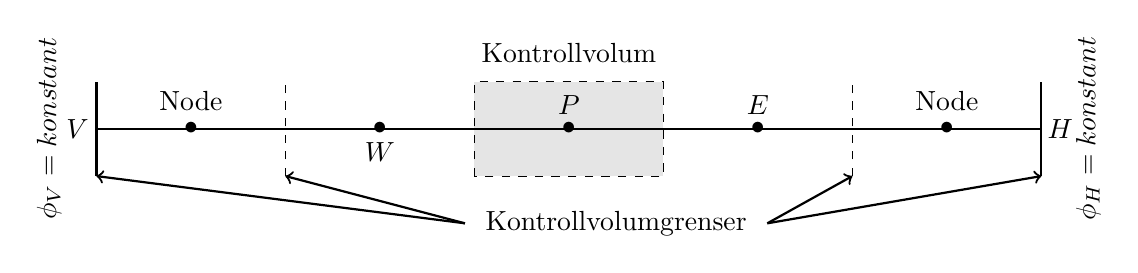
\begin{tikzpicture}[scale=1.2]
% Control volume

\draw[fill=gray!20,dashed] (2.5,0) rectangle (4.5,1); % Control volume
\draw[thick] (-1.5,.5) -- (8.5,.5);

\draw[thick] (-1.5,0) -- (-1.5,1);
\draw[thick] (8.5,0) -- (8.5,1);
\draw[thick] (0,.5) -- (8,.5);
\draw[dashed] (.5,0) -- (.5,1); % g0
\draw[dashed] (6.5,0) -- (6.5,1); % g1
% Nodes and labels
\node at (3.5,0.75) {$P$};
\node at (1.5,0.25) {$W$};
\node at (5.5,.75) {$E$};
\node at (-.5,0.5) {$\bullet$};
\node at (1.5,0.5) {$\bullet$};
\node at (3.5,0.5) {$\bullet$};
\node at (5.5,.5) {$\bullet$};
\node at (7.5,.5) {$\bullet$};

\node at (-2,0.5) [rotate=90] {$\phi_V = \text{konstant}$};
\node at (9,0.5) [rotate=90] {$\phi_H = \text{konstant}$};
\node at (-1.7,0.5) {$V$};
\node at (8.7,0.5) {$H$};

\node at (4,-0.5) {Kontrollvolumgrenser};
\draw[thick,->] (2.4,-.5) -- (.5,0);
\draw[thick,->] (2.4,-.5) -- (-1.5,0);
\draw[thick,->] (5.6,-.5) -- (6.5,0);
\draw[thick,->] (5.6,-.5) -- (8.5,0);
\node at (3.5,1.3) {Kontrollvolum};
\node at (7.5,0.8) {Node};
\node at (-.5,0.8) {Node};
\end{tikzpicture}
\caption{Skjematisk visning av kontrollvolum og nodale punkter}
\label{fig:cv-boundaries}
\end{figure}
\subsubsection*{Steg 1: Rutenettgenerering}
Det første steget i endeligvolum-metoden er å dele opp mengden i diskrete kontrollvolumer. Det gjøres på følgende vis.
\begin{enumerate}
\item Vi plasserer et antall punkter, eller noder, i rommet mellom $V$ og $H$. 
\item Grensene (eller flatene) til kontrollvolumene plasseres midt mellom nabopunkter. Hver punkt er derfor omgitt av et kontrollvolum, også kalt en celle.
\item  Det er vanlig praksis å fordele nodene slik at de fysiske randene faller sammen med kontrollvolumgrensene.
\end{enumerate}
På dette tidspunktet er det hensiktsmessig å etablere et notasjonssystem som kan brukes videre. Den vanlige konvensjonen vises i Figur~\ref{fig:grid-notation}.

\begin{figure}[ht]
\centering
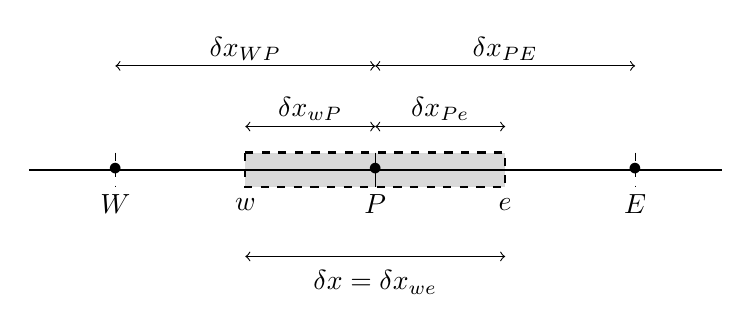
\begin{tikzpicture}[scale=1.1]

\coordinate (A) at (2.5,0.2);
  \coordinate (B) at (2.5,-0.2);
  \coordinate (C) at (5.5,-0.2);
  \coordinate (D) at (5.5,.2);


  % Draw the shaded area
  \fill[gray!30] (A) -- (B) -- (C) -- (D) -- cycle;

  % Draw the dashed border
  \draw[dashed, thick] (A) -- (B) -- (C) -- (D) -- cycle;
% Nodes
\draw[thick] (0,0) -- (8,0);
\draw[dashed] (1,0.2) -- (1,-0.2); % W
\draw[-] (4,0.2) -- (4,-0.2); % P
\draw[dashed] (7,0.2) -- (7,-0.2); % E

% Labels
\node at (1,-0.4) {$W$};
\node at (2.5,-0.4) {$w$};
\node at (4,-0.4) {$P$};
\node at (5.5,-0.4) {$e$};
\node at (7,-0.4) {$E$};
\node at (4,0) {$\bullet$};
\node at (1,0) {$\bullet$};
\node at (7,0) {$\bullet$};

% Arrows and distances
\draw[<->] (2.5,0.5) -- (4,0.5); \node at (3.25,0.7) {$\delta x_{wP}$};
\draw[<->] (1,1.2) -- (4,1.2); \node at (2.5,1.4) {$\delta x_{WP}$};
\draw[<->] (4,1.2) -- (7,1.2); \node at (5.5,1.4) {$\delta x_{PE}$};
\draw[<->] (4,0.5) -- (5.5,.5); \node at (4.75,0.7) {$\delta x_{Pe}$};
\draw[<->] (2.5,-1) -- (5.5,-1); \node at (4,-1.3) {$\delta x = \delta x_{we}$};
\end{tikzpicture}
\caption{Notasjon for én-dimensjonal gitterinndeling og kontrollvolum}
\label{fig:grid-notation}
\end{figure}

Et generelt nodalpunkt identifiseres med $P$ og naboene i én-dimensjonal geometri, nodene vest og øst, henholdsvis $W$ og $E$. Den vestlige siden av kontrollvolumet kalles «$w$» og den østlige siden «$e$». Avstandene mellom nodene $W$ og $P$, og mellom $P$ og $E$, betegnes henholodsvis $\delta x_{WP}$ og $\delta x_{PE}$. Tilsvarende betegnes avstanden mellom $W$ og flate $w$ med $\delta x_{wP}$ og mellom $P$ og flate $e$ med $\delta x_{Pe}$. Figur~\ref{fig:grid-notation} viser at kontrollvolumbredden er $\delta x = \delta x_{we}$.

\subsubsection*{Steg 2: Diskretisering}
Brorparten av arbeidet med endeligvolum-metode er integrasjon av den styrende ligningen over et kontrollvolum for å gi en diskretisert ligning ved nodalpunktet $P$. For kontrollvolumet definert gir dette:
\begin{align}\label{eV_discretisering}
\iiint_{KV} \frac{\partial}{\partial x} \left(\Gamma \frac{\partial\phi}{\partial x} \right) dV + \iiint_{KV} S dV = \left(\Gamma A \frac{\partial\phi}{\partial x}\right)_e- \left( \Gamma A \frac{\partial\phi}{\partial x} \right)_w + \tilde{S} = 0
\end{align}
Her er $A$ tverrsnittsarealet til overflaten av kontrollvolum, og $\tilde{S}$ den gjennomsnittlige verdien av $S$ ganget med volum av $KV$. 
For å utlede noe nyttig fra \eqref{eV_discretisering} trenger vi
\begin{itemize}
\item diffusjonskoeffisienten $\Gamma$ og gradienten $\nabla \phi = \frac{\partial \phi}{\partial x}$ ved øst ($e$) og vest ($w$).
\item verdier $\phi$ og $\Gamma$ bare ved nodale punkter (e.g. $P$,$W$,$W$, osv.).
\end{itemize}
For å beregne gradienter (og dermed flukser) ved kontrollvolumflater brukes en tilnærmet fordeling mellom nodale punkter. Lineære tilnærminger er den enkleste og mest åpenbare metoden, kjent som sentral differensiering.

\begin{defn}{}
Vi skal bruke subscript som notasjon for  verdier av funksjoner ved et gitt punkt. For eksempel er $\Gamma_P$ verdien til $\Gamma$ i punktet $P$.
\end{defn}

\begin{oppsum}{Tilnærming ved sentral differensiering}
 I et uniformt gitter\footnote{dette betyr at alle punkter har samme avstand fra hverandre} er interpolerte verdier:
\[
\Gamma_e = \frac{\Gamma_P + \Gamma_E}{2}, \quad \Gamma_w = \frac{\Gamma_W + \Gamma_P}{2}
\]
De diffusive fluksene evalueres som:
\[
\left( \Gamma A \frac{\partial\phi}{\partial x} \right)_e = \Gamma_e A_e \frac{\phi_E - \phi_P}{\delta x_{PE}}, \quad
\left( \Gamma A \frac{\partial\phi}{\partial x} \right)_w = \Gamma_w A_w \frac{\phi_P - \phi_W}{\delta x_{WP}}
\]
Kildetermet tilnærmes som et lineært uttrykk (vi bruker superscript for å henvise til at $S$ ikke evalueres i et punkt i formelen):
\[
\tilde{S} = S^u + S_P \phi_P
\]
\end{oppsum}
Ved å sette inn disse uttrykkene i \eqref{eV_discretisering} får vi:
\[\Gamma_eA_e\frac{\phi_E-\phi_P}{\delta x_{PE}}- \Gamma_wA_w\frac{\phi_P-\phi_W}{\delta x_{WP}}+(S^u+S_P\phi_P)\]
Vi kan nå sortere alle ledd med $\phi_P$ på venstre side og alle med $\phi_W,\phi_E$ og uten $\phi$ på høyre. Dette gir ligningen på formen
\begin{align} \label{disc_finvol1}
a_P \phi_P &= a_W \phi_W + a_E \phi_E + S^u  \\
&\text{ hvor } a_W := \frac{\Gamma_w A}{\delta x_{WP}}, \qquad a_E := \frac{\Gamma_e A}{\delta x_{PE}}, \qquad
a_P := a_W + a_E - S_P \notag
\end{align}

\subsubsection*{Steg 3: Løsning av ligninger}

Diskretiserte ligninger av formen \eqref{disc_finvol1} må settes opp ved hvert nodalpunkt for å løse problemet. For kontrollvolumer som er ved grensene av mengden, modifiseres den generelle diskretiserte ligningen for å inkludere randbetingelser. Det resulterende systemet av lineære algebraiske ligninger løses deretter for å finne fordelingen av egenskapen $\phi$ ved nodene. Enhver egnet matrise-løsningsmetode kan brukes. Sammendrag av metoden som vi skal se på i de neste to kapitler finnes i \Cref{app:EV:sammendrag}.

\begin{oppsum}{Fysisk tolkning av endelig volum metode}
Vi kan tolke \eqref{eV_discretisering} og dermed den endelige volum metode slik at den diffusive fluksen av $\phi$ som forlater den østlige flaten minus den som kommer inn fra den vestlige flaten er lik genereringen av $\phi$ – altså en bevaringslov over $KV$.
Dermed bygger endeligvolum-metode på en bevaringslov. Det skiller metoden fra endelig differanser som vi så tidligere, og som ikke automatisk oppfyller noen bevaringslov mellom forskjellige volum.
\end{oppsum}
\section{Endelig volummetode for 1D diffusjonsproblemer}\label{sect:evm1d}
I denne seksjonen anvendes den endelige volummetoden for å løse enkle diffusjonsproblemer som involverer varmeledning. Ligningen for én-dimensjonal stasjonær varmeledning er:
\begin{align}\label{1D-heateq}
\frac{\partial}{\partial x} \left( k \frac{\partial T}{\partial x} \right) + S = 0
\end{align}
hvor $k$ er varmeledningsevnen og $T$ er temperaturen.
\begin{rem}{}
Varmeledningsevne $k$ i \eqref{1D-heateq} ta plassen av koeffisient $\Gamma$ i \eqref{eV_discretisering}.

Kildetermet $S$ kan for eksempel representere varme generert av elektrisk strøm gjennom staven.
\end{rem}
 Randbetingelser og behandling av kildetermer introduseres gjennom tre eksempler.

\begin{eks}{}
\label{ex:CFD_simplest}
Betrakt problemet med varmekonduksjon uten kilde i en isolert stav med endene holdt ved konstante temperaturer på venstre $T_V := 100\,^\circ$C og $T_H:= 500\,^\circ$C på høyre. Vi skisserer det fysiske problemet:
\begin{center}
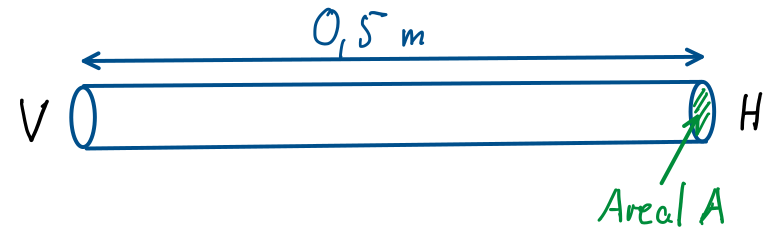
\includegraphics[width=10cm]{Fig/1Dvarme.png}
\end{center}
Tverrsnittsarealet $A$ antas å være konstant (dvs. staven er like tykk over hele lengden).
Det én-dimensjonale problemet er styrt av en forenklet versjon av \eqref{1D-heateq}:
\begin{equation}\label{eq:ex343}
\frac{\partial}{\partial x} \left( k \frac{\partial T}{\partial x} \right) = 0
\end{equation}
\end{eks}
Vi skal i det følgende løse \eqref{eq:ex343} nummerisk ved endeligvolum-metode. La oss dele staven i fem like store kontrollvolumer, noe som gir $\delta x = 0.1\,\text{m}$. 
\begin{figure}[ht]
\centering
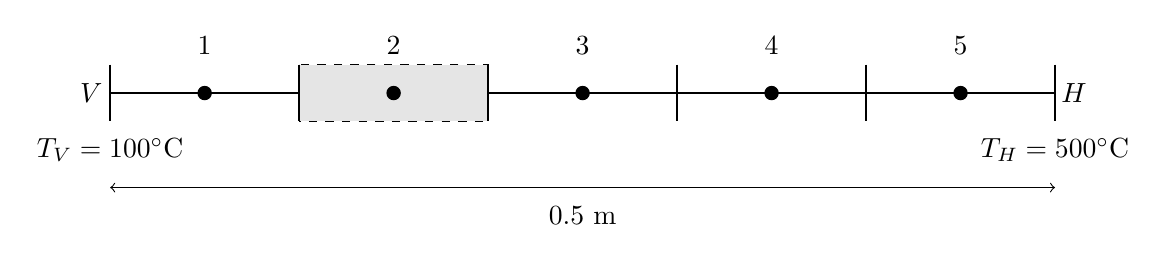
\begin{tikzpicture}[scale=1.2]

% Draw the rod
\draw[thick] (0,0) -- (10,0);

% Draw control volume divisions
\draw[fill=gray!20,dashed] (2,0.3) rectangle (4,-0.3); % Control volume

\foreach \x in {0,2,4,6,8,10} {
    \draw[thick] (\x,0.3) -- (\x,-0.3);
}

% Node labels
\node at (1,0.5) {$1$};
\node at (3,0.5) {$2$};
\node at (5,0.5) {$3$};
\node at (7,0.5) {$4$};
\node at (9,0.5) {$5$};

% Node positions
\foreach \x in {1,3,5,7,9} {
    \filldraw[black] (\x,0) circle (2pt);
}

% Boundary conditions
\node at (-.2,0) {$V$};
\node at (10.2,0) {$H$};
\node[align=center] at (0,-.6) {$T_V = 100^\circ$C};
\node[align=center] at (10,-.6) {$T_H = 500^\circ$C};

% Length annotation
\draw[<->] (0,-1) -- (10,-1);
\node at (5,-1.3) {0.5 m};
\end{tikzpicture}
\caption{Diskretisering av en 0.5 m lang stav i fem kontrollvolumer}
\end{figure}
Gitteret består av fem noder.

\paragraph{For nodene 2, 3 og 4} kan temperaturverdiene til øst og vest hentes fra nabonoder. Vi bruker nå at varmeledningsevne, arealgjennomsnitt av staven og avstand $\delta x$ er konstant. Integrasjon av \eqref{eq:ex343} over et av de indre kontrollvolum gir nå diskretiserte ligninger på følgende form:
\begin{align*}
\left(\frac{k_e}{\delta x_{PE}}A_e + \frac{k_w}{\delta x_{WP}}A_W \right)T_P &=\left(\frac{k_w}{\delta x_{WP}}A_w\right) T_W + \left(\frac{k_e}{\delta x_{PE}}A_e\right) T_E  \\
\Leftrightarrow \underbrace{\left(\frac{k}{\delta x}A + \frac{k}{\delta x}A\right)}_{=:a_P}T_P &=\underbrace{\left(\frac{k}{\delta x}A\right)}_{=:a_W} T_W + \underbrace{\left(\frac{k}{\delta x}A\right)}_{=:a_E} T_E
\end{align*}
Vi får dermed som diskretisert ligning i hver av nodene $2,3,4$ at
\begin{align}
a_P T_P = a_W T_W + a_E T_E,\quad \text{hvor } a_W = a_E = \frac{kA}{\Delta x}, \quad a_P = a_W + a_E
\end{align}
Siden det ikke finnes noen varmekilde i modellen, er $S^u = 0$ og $S_P = 0$ (se \eqref{disc_finvol1}).

\paragraph{For randnodene 1 og 5 }må vi inkludere randbetingelsene. Integrasjon av \eqref{eq:ex343} over kontrollvolum\footnote{Integralet blir et trippelintegral ettersom vi integrerer over et volum (som navn til metoden sier). Ligningen her er forresten bare avhengig av koordinat $x$ og det er det hvorfor vi kaller det et 1D-problem (selv om integralene er trippelintegraler).} med node $1$ gir 
\begin{align}\label{eq:ex343_rand}
0= \iiint_{KV} \frac{\partial}{\partial x}\left(k\frac{\partial T}{\partial x}\right) \, dV = kA\frac{T_E-T_P}{\delta x} -kA\frac{T_P-T_V}{\partial x/2}=0
\end{align}
Husk at fluks gjennom grensflaten med areal $A$ approksimeres ved en lineær relasjon mellom temperaturen ved rand $V$ og node $P$. Vi skriver nå \eqref{eq:ex343_rand} som\footnote{Husk at node $W$ eksisterer ikke siden det ligger til venstre av $V$. Vi har allerede sett bruk av fiktive punkter i randbetingelser i siste kapittel, se \Cref{ex1:RVP}}:
\begin{align}\label{eq:rand_vest}
\frac{3k}{\delta x} A T_P = 0\cdot T_W + \frac{k}{\delta x} T_E + \frac{2k}{\delta x} A T_V
\end{align}
Nå sammenlikner vi \eqref{eq:rand_vest} med \eqref{disc_finvol1} fiksert temperatur $T_V$ inkluderes som  en kilde i$(S^u+S_PT_P)$ i ligning, hvor $S^u=(2kA/\delta x)T_V$ og $S_P = -2kA/\delta x$ (mens koeffisienten for den fiktive punkt $W$ settes lik $0$).
Dermed får vi for node $1$ som gir venstre rand
\begin{align}\label{eq:ex343_rand1}
a_P T_P = a_W T_W +a_E  T_E + S^u.\notag \\ \text{hvor } a_W=0, a_E = \frac{kA}{\delta x}, a_P = a_E - S_P  \quad S^u = \frac{2kA}{\delta x} T_V, \ S_P = -\frac{2kA}{\delta x}. 
\end{align}
Tilsvarende for node $5$, med kjent temperatur $T_H$:
\begin{align}\label{eq:ex343_rand5}
a_P T_P = a_W T_W + a_E T_E + S^u, \notag\\ 
\text{hvor } a_W=\frac{kA}{\delta x}, a_E = 0, a_P = a_W +a_E - S_P  \quad S^u = \frac{2kA}{\delta x} T_H, \ S_P = -\frac{2kA}{\delta x},
\end{align}
Ved å sette inn numeriske verdier $kA/\delta x = 100$ man kan bestemme koeffisienter:
\begin{center}
\begin{tabular}{|c|c|c|c|c|c|}
\hline
Node & $a_W$ & $a_E$ & $S^u$ & $S_P$ & $a_P=a_W+a_E-S_P$ \\
\hline
$1$ & $0$ & $100$ & $200T_V$ & $-200$ & $300$ \\
$2$ & $100$ & $100$ &  $0$ &  $0$ & $200$ \\
$3$ & $100$ & $100$ &  $0$ &  $0$ & $200$ \\
$4$ & $100$ & $100$ &  $0$ &  $0$ & $200$ \\
$5$ & $100$ & $0$ & $200T_H$ & $-200$ & $300$ \\
\hline
\end{tabular}
\end{center}
Dette resulterer i følgende ligningssystem for temperaturene i noder (se Python notat for matrise versjon av ligningssystemet):
\[
\begin{aligned}
300 T_1 &= 100 T_2 + 200 T_V \\
200 T_2 &= 100 T_1 + 100 T_3 \\
200 T_3 &= 100 T_2 + 100 T_4 \\
200 T_4 &= 100 T_3 + 100 T_5 \\
300 T_5 &= 100 T_4 + 200 T_H
\end{aligned}
\]
Løsningen for $T_V = 100\,^\circ$C og $T_H = 500\,^\circ$C er:
\[
T_1 = 140, \quad T_2 = 220, \quad T_3 = 300, \quad T_4 = 380, \quad T_5 = 460
\]
Den eksakte løsningen er en lineær temperaturfordeling: $T(x) = 800x + 100$. 


Vi ser nå på et problem som inkluderer interne varmekilder, i tillegg til randbetingelser.

\begin{eks}{}\label{ex:CFD_2nd}\mbox{}
\begin{minipage}{7cm}
Figuren til høyre viser en stor plate med tykkelse $L = 2\,\text{cm}$, konstant varmeledningsevne $k = 0.5\,\text{W/}\text{m}\text{/K}$ og jevn varmegenerering $q = 1000\,\text{kW/m}^3$. Flatene $V$ og $H$ er holdt ved temperaturene $T_V = 100^\circ$C og $T_H = 200^\circ$C. 

Vi antar at dimensjonene i $y$- og $z$-retningene er så store at signifikante temperaturgradienter kun opptrer i $x$-retningen. Dermed har vi igjen et problem i én romlig dimensjon. Styrelikningen blir
\[
\frac{\partial}{\partial x} \left( k \frac{\partial T}{\partial x} \right) + q = 0
\]
Vi skal igjen diskretisere og fremstille løsning som i tidligere eksempel. Notasjon introdusert der (for noder, øst, vest etc. er fortsatt i bruk).
\end{minipage} \quad
\begin{minipage}{6cm}
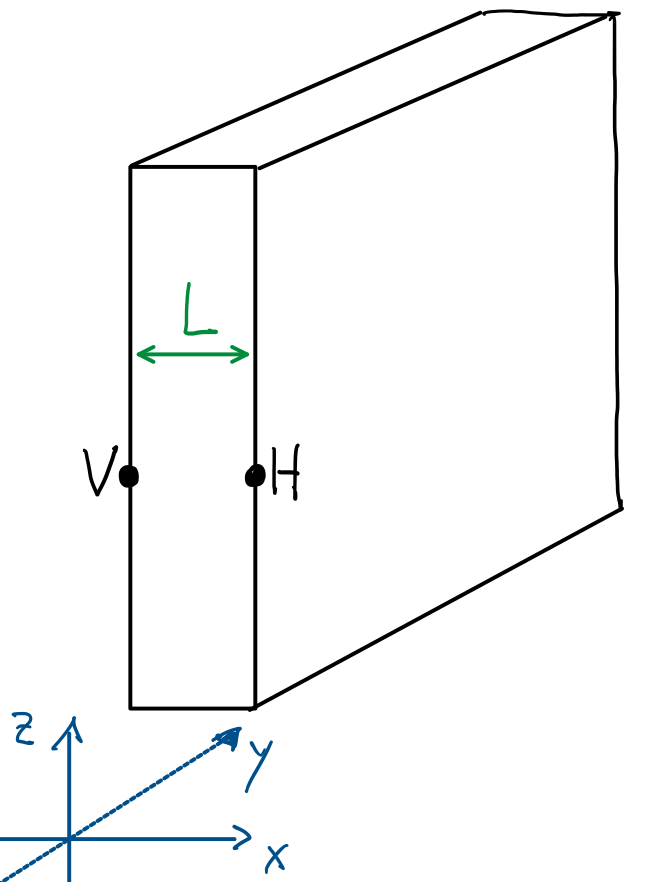
\includegraphics[width=6cm]{Fig/varmeflate.png}
\end{minipage}
\end{eks}
Som tidligere deler vi $x$-retning inn i fem kontrollvolumer $KV$, med $\delta x = 0.004\,\text{m}$. Vi antar en enhetsflate i $yz$-planet med areal $A$.
Ved formell integrasjon av den ligningen over et kontrollvolum får vi:
\begin{align}\label{ex:2_KV_int}
\iiint_{KV} \frac{\partial}{\partial x} \left(k \frac{\partial T}{\partial x}\right) dV + \iiint_{KV} q dV =0
\end{align}
Første ledd i \eqref{ex:2_KV_int} behandles som i \Cref{ex:CFD_simplest}. For det andre integralet, kilde i ligningen er evaluert ved gjennomsnittlige produksjon (dvs. $\overline{S} |KV|=q|KV|=qA\delta x$ hvor $|KV|$ betegnes volummål til kontroll volum $KV$) i hver kontrollvolum. Dermed får vi fra \eqref{ex:2_KV_int}
\[
0 = \left[ kA \frac{dT}{dx} \right]_e - \left[ kA \frac{dT}{dx} \right]_w + q |KV| = k_e A\frac{T_E-T_P}{\delta x}-k_w A\frac{T_P.T_W}{\delta x} + qA \delta x
\]
Vi kan sortere ligningen og skrive den som
\[\frac{k_e+k_w}{\delta x}AT_P = \frac{k_e}{\delta x}AT_W+ \frac{k_w\delta x}AT_E + qA\delta x\]
Husk at $k_e=k_w=k$ og dermed er ligningen for indre noder ($2$, $3$ og $4$):
\begin{align}\label{ex2:CFD_indre_eq}
a_P T_P = a_W T_W + a_E T_E + S^u\\
a_W=a_E=\frac{kA}{\delta x}, \quad a_P = a_w + a_E-S_P, \quad S_P=0,\quad  S^u= qA\delta x\notag
\end{align}
\textbf{Randbetingelser} Vi bruker for noder $1$ og $5$ igjen en liner approksimasjon for temperaturen mellom randpunkt og nabonode. Ved node $1$, med kjent temperatur $T_V$, integrasjon av ligningen over kontrollvolumet rundt node $1$ gir oss sammen med lineær approksimasjon for temperatur mellom $V$ og $P$:
\[kA \left(\frac{T_E-T_P}{\delta x}- \frac{T_P-T_V}{\delta x/2}\right)+qA\delta x=0\]
Dermed er diskretisert ligning ved randnode $1$ gitt som  
\begin{align}
a_P T_P = a_WT_W + a_E T_E + S^u\\
a_W = 0, \quad a_E = \frac{kA}{\delta x}, \quad a_P = a_E - S_P, \quad S_P = -\frac{2kA}{\delta x}, \quad S^u = \frac{2kA}{\delta x} T_V + q A \delta x, \notag
\end{align}
Ved node $5$, med kjent temperatur $T_H$, får vi lignende:
\begin{align}
a_P T_P = a_W T_W + a_ET_E + S^u\\
a_W = \frac{kA}{\delta x}, \quad a_E = 0, \quad a_P = a_W +a_E- S_P, \quad S_P = -\frac{2kA}{\delta x},    \quad S^u = \frac{2kA}{\delta x} T_H + q A \delta x, \notag
\end{align}
\textbf{Numerisk løsning}
Setter vi inn verdiene $k = 0.5$, $A = 1$, $q = 1000\,\text{kW/m}^3 = 10^6\,\text{W/m}^3$, $\delta x = 0.004\,\text{m}$, får vi:
\begin{center}
\begin{tabular}{|c|c|c|c|c|c|}
\hline
Node & $a_W$ & $a_E$ & $S^u$ & $S_P$ & $a_P=a_W+a_E-S_P$ \\
\hline
$1$ & $0$ & $125$ & $4000+250T_V$ & $-250$ & $375$ \\
$2$ & $125$ & $125$ &   $4000$ &  $0$ & $250$ \\
$3$ & $125$ & $125$ &   $4000$ &  $0$ & $250$ \\
$4$ & $125$ & $125$ &   $4000$ &  $0$ & $250$ \\
$6$ & $125$ & $0$ &  $4000 + 250T_H$ & $-250$ & $375$ \\
\hline
\end{tabular}
\end{center}
Ligningssystemet i matriseform blir:
\[
\begin{bmatrix}
375 & -125 & 0 & 0&0 \\
-125 & 250 & -125 & 0 & 0 \\
0& -125& 250 & -125 & 0\\
0&0&-125& 250 &-125 \\
0&0&0&-125&375
\end{bmatrix}
\begin{bmatrix} T_1 \\ T_2 \\ T_3 \\ T_4 \\ T_5 \end{bmatrix} = \begin{bmatrix} 
29000\\ 4000 \\ 4000 \\ 4000 \\ 54000\end{bmatrix}
\]
Løsningen (målt i kW! ikke i W) er:
\[
T_1 = 150, \quad T_2 = 218, \quad T_3 = 254, \quad T_4 = 258, \quad T_5 = 230
\]

\subsubsection*{Sammenligning med analytisk løsning}

Den analytiske løsningen finnes ved å integrere den styrende ligningen to ganger og bruke randbetingelsene:
\[
T(x) = \left(\frac{T_H - T_V}{L}  + T_V + \frac{q}{2k}(L-x)\right) x + T_V
\]
Sammenligning viser at den numeriske løsningen stemmer godt overens med den analytiske, selv med et grovt gitter.


I neste eksemplet ser vi på kjøling av en sirkulær ribbe ved hjelp av konvektiv varmeoverføring langs dens lengde. Konveksjon gir opphav til et temperaturavhengig varmetap, eller synkledd, i den styrende ligningen.
\begin{eks}{}
\Cref{fig:ribbe} viser en sylindrisk ribbe med konstant tverrsnittsareal $A$. Basen er ved temperatur $T_V = 100^\circ$C, og enden er isolert.\footnote{Isolert betyr at ingen varmeflyt skjer gjennom denne randen. Dette betyr at den deriverte av temperaturen i denne retningen forsvinner ved randen som er isolert!} Ribben er utsatt for en omgivelsestemperatur på $T_\infty = 20^\circ$C. 

Én-dimensjonal varmeoverføring i denne situasjonen styres av:
\begin{align*}
\frac{\partial}{\partial x} \left( kA \frac{\partial T}{\partial x} \right) - hO(T - T_\infty) = 0
\end{align*}
hvor $h$ er den konvektive varmeoverføringskoeffisienten til luft\footnote{Dette er altså ikke konveksjon inne i staven. Tanken er at luften rundt staven (/ribben) kjøler staven ved at konveksjonsstrømmer oppstår i luften. Luften rett rundt staven varmes opp av staven og denne varme luften transporteres så vekk ved konveksjon, altså luftstrømmer. På den måten forblir luften rett rundt staven på en konstant temperatur $20^\circ\textrm{C}$.}, $O$ er omkretsen, og $k$ er varmeledningsevnen. Den analytiske løsningen er gitt ved:
\begin{align}\label{eq:loes_ribbe}
\frac{T(x) - T_\infty}{T_V - T_\infty} = \frac{\cosh\left(n(L - x)\right)}{\cosh(nL)}
\end{align}
hvor $n^2 = \frac{hO}{kA} = 25m^{-2}$ (husk at $k,A$ er konstant!) og $L = 1\,\text{m}$ (lengde av ribbe), $x$ distanse på ribben.

Siden $k,A$ er konstant kan vi omskrive ligningen som styrer prosess som
\begin{align}\label{styr_eq_ribbe}
\frac{\partial^2T}{\partial^2 x} - n^2 (T-T_\infty)=0
\end{align}
\end{eks}
\begin{figure}[ht]
\centering
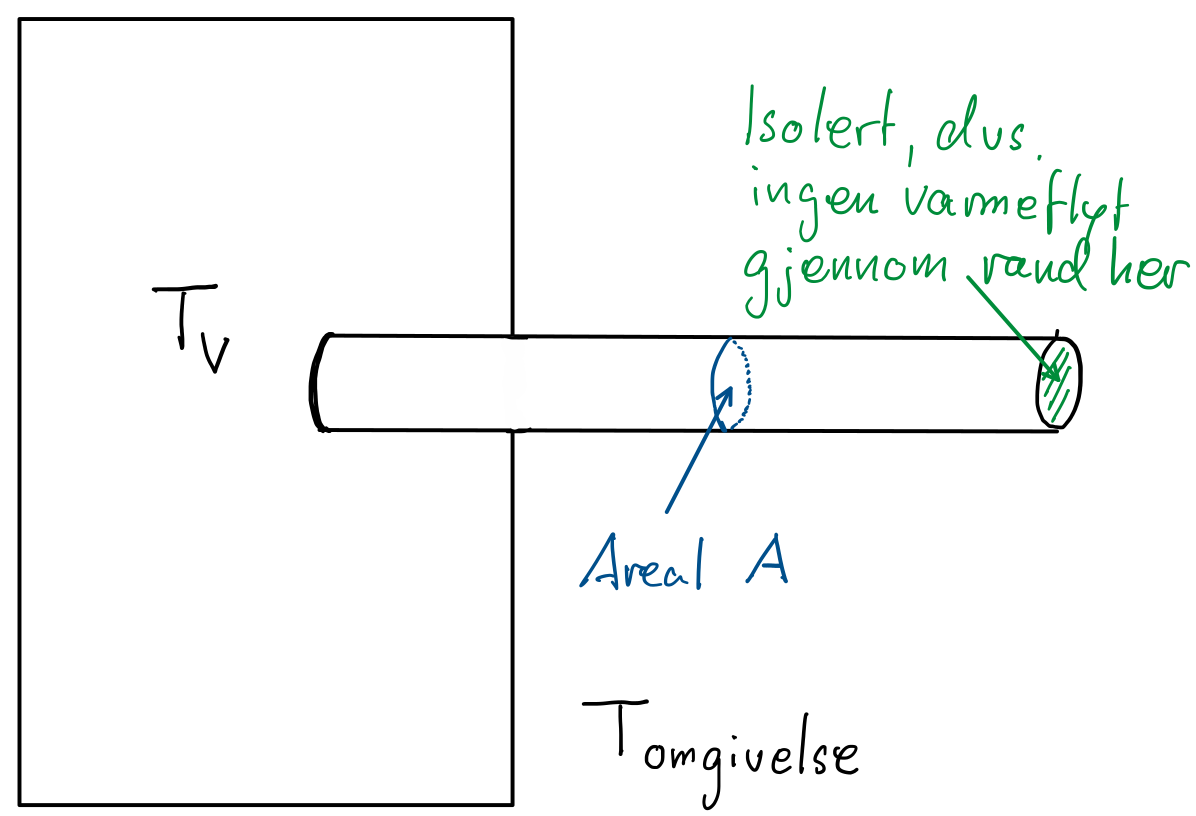
\includegraphics[width=8cm]{Fig/ribbe.png}
\caption{Kjøling av en sylindrisk ribbe.}\label{fig:ribbe}
\end{figure}
\textbf{Diskretisering for \Cref{styr_eq_ribbe}}
Ligningen \eqref{styr_eq_ribbe} har nå en ledd $-n^2(T-T_\infty)$ som slukker varme, konvektiv varmetap, som er en funksjon av temperaturen $T$. Som i tidligere eksempler lager vi en gitter. Del ribben inn i fem kontrollvolumer $KV$ med uniformt størrelse, $\delta x = 0.2\,\text{m}$.

Ved integrasjon av \eqref{styr_eq_ribbe} over et kontrollvolum får vi 
\[\iiint_{KV} \frac{\partial^2 T}{\partial x^2}\, dV - \iiint_{KV}n^2(T-T_\infty) \, dV=0\]
hvor det første integralet behandles som i \Cref{ex:CFD_simplest}. Andre integraket evalueres ved antagelse at integralet er lokalt konstant på hvert kontrollvolumen.
\[A\left(\frac{\partial T}{\partial x}\right)_e -A\left(\frac{\partial T}{\partial x}\right)_w - n^2(T_P-T_\infty)\delta x=0.\]
Vi skriver det om ved bruk av  en lineær tilnærming og får indre noder ($2, 3$ og $4$):
\begin{align*}
a_P T_P = a_W T_W + a_E T_E + S^u\\
a_W = a_E = \frac{1}{\delta x}, \quad a_P = a_W + a_E - S_P, \quad S_P = -n^2 \delta x, \quad S^u = n^2 \delta x T_\infty.
\end{align*}
\textbf{Randbetingelser}
Vi foregår akkurat som i \Cref{ex:CFD_simplest}. Ved node $1$, med kjent temperatur $T_V$, får vi:
\begin{align*}
\frac{T_E-T_P}{\delta x}-\frac{T_P-T_V}{\delta x/2}-n^2(T_P-T_\infty)\delta x=0
\end{align*}
og dette betyr at verdier for koeffisienter er gitt som
\[
a_W = 0, \quad a_E = \frac{1}{\delta x},\quad a_P = a_W+a_E-S_P, \quad S_P = -2n^2 \delta x - \frac{2}{\delta x}, \quad S^u = n^2 \delta x T_\infty + \frac{2}{\delta x} T_V, 
\]
Ved node $5$, med isolert ende (null fluks), får vi: som ligning
\begin{align*}
0-\frac{T_P-T_V}{\delta x/2}-n^2(T_P-T_\infty)\delta x=0
\end{align*}
Dermed er koeffisienter gitt som
\[
a_W=\frac{1}{\delta x}, \quad a_E = 0,\quad a_P=a_W+a_E-S_P, \quad S_P = -n^2 \delta x, , \quad S^u = n^2 \delta x T_\infty.
\]
\textbf{Numerisk løsning}
Med $n^2 = 25\,\text{m}^{-2}$ og $\delta x = 0.2\,\text{m}$, får vi:
\begin{center}
\begin{tabular}{|c|c|c|c|c|c|}
\hline
Node & $a_W$ & $a_E$ & $S^u$ & $S_P$ & $a_P=a_W+a_E-S_P$ \\
\hline
$1$ & $0$ & $5$ & $100+10T_V$ & $-15$ & $20$ \\
$2$ & $5$ & $5$ &   $100$ &  $-5$ & $15$ \\
$3$ & $5$ & $5$ &   $100$ &  $-5$ & $15$ \\
$4$ & $5$ & $5$ &   $100$ &  $-5$ & $15$ \\
$6$ & $5$ & $0$ &  $100$ & $-5$ & $10$ \\
\hline
\end{tabular}
\end{center}
Ligningssystemet i matriseform blir:
\[
\begin{bmatrix}
20 & -5 & 0 & 0&0 \\
-5 & 15 & -5 & 0 & 0 \\
0& -5& 15 & -5 & 0\\
0&0&-5& 15 &-5 \\
0&0&0&-5&10
\end{bmatrix}
\begin{bmatrix} T_1 \\ T_2 \\ T_3 \\ T_4 \\ T_5 \end{bmatrix} = \begin{bmatrix} 
1100\\ 100 \\ 100 \\ 100 \\ 100\end{bmatrix}
\]
Løsningen er:
$
T_1 = 64.22, T_2 = 36.91, T_3 = 26.50, T_4 = 22.60, T_5 = 21.30
$

\subsubsection*{Sammenligning med analytisk løsning}

Den analytiske løsningen viser god overensstemmelse med den numeriske, selv med et grovt gitter. Feilen er under 6\%.


\section{Endelig volummetode for 2D diffusjonsproblemer}\label{EVM2D}
Metodikken brukt for å utlede diskretiserte ligninger i én-dimensjonale tilfeller kan enkelt utvides til to-dimensjonale problemer. For å illustrere teknikken, vurder den to-dimensjonale stasjonære diffusjonsligningen:
\begin{align}\label{EV:2Dligning}
\frac{\partial}{\partial x} \left( \Gamma \frac{\partial \phi}{\partial x} \right) + \frac{\partial}{\partial y} \left( \Gamma \frac{\partial \phi}{\partial y} \right) + S = 0
\end{align}
Et utsnitt av det to-dimensjonale gitteret som brukes for diskretisering er vist i \Cref{2Dgrid}
\begin{figure}[ht]\centering
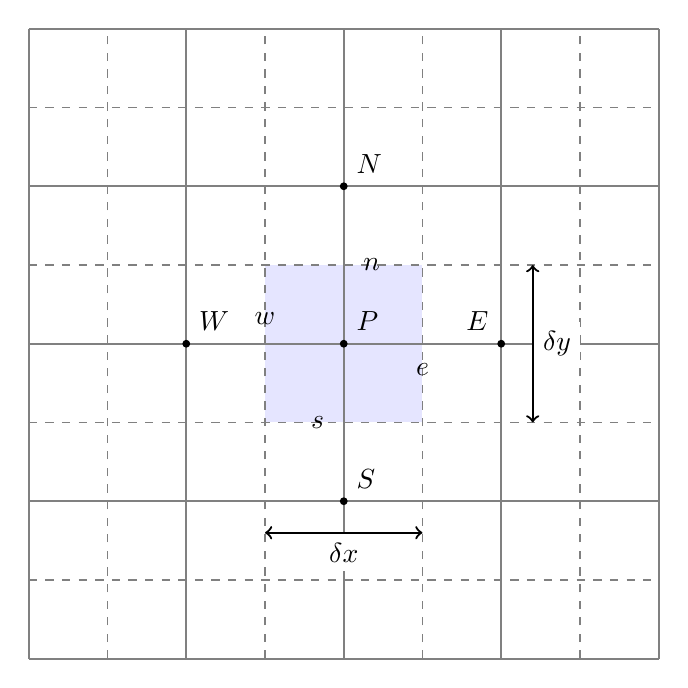
\begin{tikzpicture}
  \def\gridSize{8}
  \def\step{1}
 % Shade the 2x2 box between dashed lines (e.g., x=3 to 5, y=3 to 5)
  \fill[blue!10] (3,3) rectangle (5,5);
  % Draw vertical grid lines
  \foreach \x in {0,\step,...,\gridSize} {
    \ifodd\x
      \draw[dashed, gray] (\x,0) -- (\x,\gridSize);
    \else
      \draw[thick, gray] (\x,0) -- (\x,\gridSize);
    \fi
  }

  % Draw horizontal grid lines
  \foreach \y in {0,\step,...,\gridSize} {
    \ifodd\y
      \draw[dashed, gray] (0,\y) -- (\gridSize,\y);
    \else
      \draw[thick, gray] (0,\y) -- (\gridSize,\y);
    \fi
  }

  % Mark center points of KV and label them 
  \node[circle, fill=black, inner sep=1pt, label=above right:$P$] at (4,4) {};
  \node[circle, fill=black, inner sep=1pt, label=above right:$N$] at (4,6) {};
   \node[circle, fill=black, inner sep=1pt, label=above right:$S$] at (4,2) {};
    \node[circle, fill=black, inner sep=1pt, label=above right:$W$] at (2,4) {};
     \node[circle, fill=black, inner sep=1pt, label=above left:$E$] at (6,4) {};

  %Mark faces
  \node[label= right:$n$] at (4,5) {};
   \node[label= left:$s$] at (4,3) {};  
   \node[label= below:$e$] at (5,4) {};
   \node[label= above:$w$] at (3,4) {};  
  % Draw double-headed arrow for delta x
  \draw[<->,thick] (3,1.6) -- (5,1.6) node[midway, below,fill=white] {$\delta x$};

  % Draw double-headed arrow for delta y
  \draw[<->,thick] (6.4,3) -- (6.4,5) node[midway, right,fill=white] {$\delta y$};
\end{tikzpicture}
\caption{Notasjon og konvensjoner for en to dimensjonalt gitter. Kontrollvolum rundt $P$ er blått området.}\label{2Dgrid}
\end{figure}
I tillegg til østlige ($E$) og vestlige ($W$) naboer, har et generelt gitterpunkt $P$ nå også nordlige ($N$) og sørlige ($S$) naboer. Samme notasjon som i én-dimensjonal analyse brukes for flater og celledimensjoner. Spesielt skriver vi $s,e,n,w$ for rand av kontrollvolum i retning av naboene $S,E,N$ og $W$.

Ved formell integrasjon av \eqref{EV:2Dligning} over et kontrollvolum får vi:
\begin{align}
\iiint_{KV} \frac{\partial}{\partial x} \left( \Gamma \frac{\partial \phi}{\partial x} \right) dV + \iiint_{KV} \frac{\partial}{\partial y} \left( \Gamma \frac{\partial \phi}{\partial y} \right) dV + \iiint_{KV} S dV = 0
\end{align}
Siden gitteren er uniform i hver romdimensjon får vi $A_w = A_e = \delta y$ konstant. Lignende for nord og sør er $A_n = A_s = \delta x$. Dermed forenkles ligningen som
\[
\Gamma_e  A_e\left(\frac{\partial \phi}{\partial x}\right)_e - \Gamma_w A_w \left(\frac{\partial \phi}{\partial x}\right)_w  + \Gamma_n A_n\left(\frac{\partial \phi}{\partial x}\right)_n - \Gamma_s  A_s\left(\frac{\partial \phi}{\partial x}\right)_s  + \overline{S} |KV| = 0
\]
Som tidligere representerer det en bevaringslov som balanserer generering av $\phi $ i en kontrollvolum og fluksene over randene av volumet. Igjen får vi som tilnærming
\[\text{Fluks over }w: \Gamma_w A \left(\frac{\partial \phi}{\partial x}\right)_w =\Gamma_w A\frac{\phi_P-\phi_W}{\delta x_{WP}}\]
og så videre for de andre randflater. Setter vi det inn i ligningen over får vi
\begin{align}
\Gamma_e A_e \frac{\phi_E - \phi_P}{\delta x_{PE}} - \Gamma_w A_w \frac{\phi_P - \phi_W}{\delta x_{WP}} + \Gamma_n A_n \frac{\phi_N - \phi_P}{\delta y_{PN}} - \Gamma_s A_s \frac{\phi_P - \phi_S}{\delta y_{SP}} + \overline{S} |KV| = 0
\end{align}
Når kildetermet representeres i lineær form $\overline{S} |KV| = S^u + S_P \phi_P$, kan ligningen omskrives som:
\begin{align*}
a_P \phi_P = a_W \phi_W + a_E \phi_E + a_S \phi_S + a_N \phi_N + S^u\\
a_W = \frac{\Gamma_w A_w}{\delta x_{WP}}, \quad
a_E = \frac{\Gamma_e A_e}{\delta x_{PE}}, \quad
a_S = \frac{\Gamma_s A_s}{\delta y_{SP}}, \quad
a_N = \frac{\Gamma_n A_n}{\delta y_{PN}}, \\
a_P = a_W + a_E + a_S + a_N - S_P
\end{align*}
For å finne fordelingen av $\phi$ i en gitt to-dimensjonal situasjon, skrives diskretiserte ligninger av denne formen for hvert gitterpunkt i det delte domenet.

Ved randen, der temperaturer eller flukser er kjent, modifiseres ligningene for å inkludere randbetingelser på samme måte som vist i \Cref{ex:CFD_simplest}. Koeffisienten på randsiden settes til null (koblingen kuttes), og fluksen over randen legges til som en kilde i $S^u$ og $S_P$. Observer at nye koeffisienter i $2D$-problemer er bare avhengig av nabopunktene, dvs. hvis vi leter etter koeffisient i punkt $P$ trenger vi også verdier i nabopunkter $W,E,N,S$. Dette gir et mønstret som er kjent som $5$-punkt stencil vist i \Cref{5pt_stencil}.
\begin{figure}[ht!]\centering 
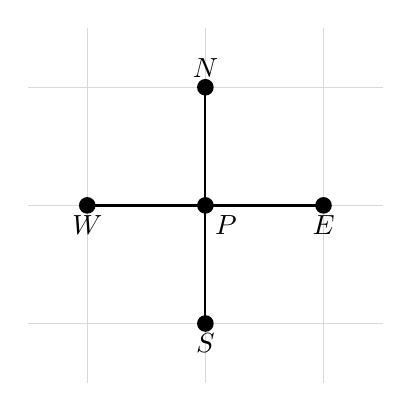
\begin{tikzpicture}[scale=1.5]

% Coordinates
\coordinate (P) at (0,0);
\coordinate (W) at (-1,0);
\coordinate (E) at (1,0);
\coordinate (N) at (0,1);
\coordinate (S) at (0,-1);

% Draw grid lines for context
\draw[step=1cm,gray!30,thin] (-1.5,-1.5) grid (1.5,1.5);

% Draw points
\fill (P) circle (2pt);
\fill (W) circle (2pt);
\fill (E) circle (2pt);
\fill (N) circle (2pt);
\fill (S) circle (2pt);

% Labels
\node[below right] at (P) {$P$};
\node[below] at (W) {$W$};
\node[below] at (E) {$E$};
\node[above] at (N) {$N$};
\node[below] at (S) {$S$};

% Optional: connect points to P
\draw[thick] (P) -- (W);
\draw[thick] (P) -- (E);
\draw[thick] (P) -- (N);
\draw[thick] (P) -- (S);

\end{tikzpicture}\caption{Mønstret som er kjent som Fem punkt stencil.}\label{5pt_stencil}
\end{figure}

Det resulterende ligningssystemet løses for å finne den to-dimensjonale fordelingen av $\phi$. 

\section{Ligninger som inkluderer en tidsparameter}

Etter å ha betraktet statiske ligninger i de siste eksempler, skal vi nå forklare hvordan en ikke-statisk ligning kan behandles i diskretiseringen. Dette gjøres ved å betrakte tidsparameteren som en ekstra dimensjon i diskretiseringen, slik at vi får et skjema som utvikler løsningen i tid.

Vi betrakter den tidsavhengige varmeledningslikningen i to dimensjoner:
\begin{align}\label{eq:varme_tid}
u_t = u_{xx} + u_{yy}, \quad (x,y) \in \Omega, \; t > 0.
\end{align}
For å diskretisere i tid bruker vi en fremover differanse:
\[
\frac{u^{n+1}_{i,j} - u^n_{i,j}}{\delta t} \approx u_t(x_i,y_j,t^n).
\]
Her er $i,j$ parametrer vi bruker for diskretisering i rom, mens $n$ brukes som diskretiseringsparameter i tidsretning.

Deretter kan vi ordne ligningen \eqref{eq:varme_tid} på nytt slik at
\[u_{i,j}^{n+1} = u_{i,j}^n + \delta t (u_{xx} + u_{yy})\]
Vi må nå diskretisere $u_{xx}$ og $u_{yy}$ men vitsen med formelen er at det eneste ledd i formelen som er avhengig av $t_{n+1}$ (neste tidssteg) er på venstre side av formelen. Alle ledd på høyre side er faktisk bare avhengig av $t_n$.

Vi kan nå kjøre en diskretiseringsskjema (enten endelige differanser eller endelig volum metode for ligningen på høyre). 

\subsubsection*{Eksempel: Endelige differanser}
For eksemepel hvis vi bruker endelige differanser får vi det følgende: 
Romlige deriverte diskretiseres med sentraldifferanser:
\[
u_{xx} \approx \frac{u^n_{i+1,j} - 2u^n_{i,j} + u^n_{i-1,j}}{\delta x^2}, \qquad
u_{yy} \approx \frac{u^n_{i,j+1} - 2u^n_{i,j} + u^n_{i,j-1}}{\delta y^2}.
\]
Setter vi dette sammen, får vi den eksplisitte skjemaet:
\[
u^{n+1}_{i,j} = u^n_{i,j} + \delta t \left(
\frac{u^n_{i+1,j} - 2u^n_{i,j} + u^n_{i-1,j}}{\delta x^2} +
\frac{u^n_{i,j+1} - 2u^n_{i,j} + u^n_{i,j-1}}{\delta y^2}\right)
\]
Dette er et \emph{fremover-Euler} skjema i tid og ligningen fører til utvidelse av \emph{fem-punkts stencil} \Cref{5pt_stencil} i rom. 

\subsubsection{Eksempel: Endelig volum metode}

Vi har allerede sett på diskretisering av 
$$u_{xx}+u_{yy}=0$$
ved hjelp av EVM siden det samsvarer \eqref{EV:2Dligning} for $\Gamma \equiv 1$ og $S\equiv 0$ fra \Cref{EVM2D}. Dermed kunne vi bruke koeffisientene som er utviklet det for å utlede en EVM-basert diskretisering av 2D-ligning. Setter vi alt sammen får vi igjen en utvidelse av 5 punkt stencil for en tilleggs-tidsparameter,

I \Cref{timdep_stencil} viser vi fremgangsmåte og hvordan neste tidssteg er avhengig av fem punkter i rom for tid $t_n$ (det gjelder både EDM og EVM fremgangsmåte).



\begin{figure} \centering
\begin{tikzpicture}[scale=2, x={(1cm,0cm)}, y={(0.5cm,0.5cm)}, z={(0cm,1cm)}]

% Define stencil points in xy-plane (z=0)
\coordinate (C) at (0,0,0);    % center
\coordinate (N) at (0,1,0);    % north
\coordinate (S) at (0,-1,0);   % south
\coordinate (E) at (1,0,0);    % east
\coordinate (W) at (-1,0,0);   % west

% Next time step point along z-axis
\coordinate (T) at (0,0,1.2);

% Draw axes
\draw[->] (-1.8,0,0) -- (1.8,0,0) node[right] {$x$};
\draw[->] (0,-1.8,0) -- (0,1.8,0) node[above] {$y$};
\draw[->] (0,0,0) -- (0,0,1.8) node[above] {$t$};

% Draw wider grid in xy-plane
\foreach \i in {-2,-1,0,1,2} {
    \foreach \j in {-2,-1,0,1,2} {
        \fill[gray!40] (\i,\j,0) circle (0.8pt);
    }
}

% Highlight stencil points
\foreach \p/\lbl in {C/$u^n_{i,j}$, N/$u^n_{i,j+1}$, S/$u^n_{i,j-1}$, E/$u^n_{i+1,j}$, W/$u^n_{i-1,j}$} {
    \fill[black] (\p) circle (2pt);
    \node[below right] at (\p) {\lbl};
}

% Draw next time step point
\fill[red] (T) circle (2pt);
\node[right] at (T) {$u^{n+1}_{i,j}$};

% Connect stencil points to next time step with dashed blue lines
\foreach \p in {C,N,S,E,W} {
    \draw[blue, dashed, thick] (\p) -- (T);
}
\end{tikzpicture}\caption{Fem punkt stencil og diskretisering av en tidsavhengig ligning.}\label{timdep_stencil}
\end{figure}